% <preamble>
\documentclass[12pt,a4paper,dvips]{article}
\usepackage{graphicx,xspace,overcite,amsmath}

\usepackage[dvips,
	bookmarks,
	colorlinks=true,
	hyperindex=true,
	hyperfigures,
	bookmarksnumbered=true]{hyperref}

\def\mydash{${-}$}
\newcommand{\D}{\displaystyle}
\newcommand{\etal}{{\it et al.}}
\sloppy

% </preamble>
% <document>
% <frontpage>
\begin{document}
\title{GMIN User Guide}
\author{David J.~Wales}
\date{Last updated \today}
\maketitle

\clearpage
\phantomsection
\pdfbookmark[0]{\contentsname}{contents} % Sets a PDF bookmark for the Table of Contents
\tableofcontents
% </frontpage>
% <intro>
\section{Introduction}

GMIN is a program that attempts to find the global potential energy minimum
for a collection of atoms or molecules using the `basin-hopping' algorithm
described by Wales and Doye.\cite{walesd97a}
A constant temperature Monte Carlo (MC) run is performed on the transformed
potential energy surface (PES), and the configuration point may either be reset 
to the latest minimum in the chain or vary freely.
The program knows many different empirical potentials and it is straightforward to add new systems.
From version 2.2 basin-sampling thermodynamics has been added, and from 
version 2.3 parallel tempering basin-sampling and basin-hopping have been
implemented with MPI.

To start a calculation, you need a file called {\tt data} in the current directory,
along with a file called {\tt coords} containing the initial coordinates,
which can be random. If the {\it SEED} keyword is present in
{\tt data} you also need a file called {\tt seed} containing the seed coordinates.
Most output is written to a file called {\tt output} (the filename can be changed by giving the 
new name as an argument to the GMIN executable). The file {\tt lowest} is always created
at the end of the run, containing the energies and geometries of the lowest few
configurations found in the given run. The geometries are saved in XMakemol xyz format.

\section{Installation}

GMIN has been tested on most Linux distributions with the nagfor, ifort, pgf90,
pathscale, and g77 compilers.
Other operating systems are not supported.
The source is available as a compressed tarball from URL www-wales.ch.cam.ac.uk/GMIN/.

To install GMIN first uncompress and unpack the tarball. Then, if you are using CMake to build 
the executables, see the README file within the directory structure you just unpacked.
Alternatively, if you are (still) using make, cd to the GMIN/source directory 
and edit the Makefile to uncomment the options for your chosen compiler. The blocks
for other compilers should be commented. After make clean and make this should produce
an executable in the GMIN/bin directory.

\section{History}

From version 2 onwards GMIN was recoded in fortran90. 
Dynamic memory allocation is now used, so there are no hard limits on parameters
such as the number of atoms.
A number of new keywords have also been added since the first version of the code,
as well as numerous potentials.
The most important are probably {\it SYMMETRY}, {\it AVOID}, and {\it COOPMOVE}, which 
are directly used in global optimisation, 
and {\it HISTOGRAM}, which specifies a `basin-sampling' calculation of the energy
density of states.
A new algorithm (bipartite matching) has also been introduced for use with {\it PERMDIST}
and {\it AVOID} to deal with permutational isomers.
The implementation of {\it PERMDIST} is now the same as in OPTIM
and PATHSAMPLE, with a {\tt perm.allow} file to specify groups of permutable
atoms and secondary sets that can only permute together.
Finally, GMIN has been interfaced with CHARMM in much the same way as OPTIM, and there
are new keywords to specify how the current geometry should be perturbed in the
step-taking process. Keyword {\it CHARMMTYPE} specifies the type of CHARMM potential,
while {\it CHPMAX}, {\it CHPMIN}, {\it CHNMAX}, {\it CHNMIN},
{\it NOPHIPSI}, and {\it TOMEGA} govern the step-taking procedure in {\bf charmmgmin.src}.
Keyword {\it INTMIN} specifies that minimisation should be performed in internal coordinates,
but this seems to be slower than Cartesian coordinates in general.

Also new from version 2.3, the global minimisation basin-hopping algorithm has been enhanced with a 
parallel tempering option, which is implemented using MPI. Please see the notes
in the Makefile when loading compilers and MPI libraries. 
(Note that the LAM MPI 32-bit library is currently broken! MPICH has not been tested yet.)
The keyword {\it MPI} specifies
the number of processors for the parallel job and {\it BHPT} allows the user to specify the temperature
range over which the replicas are exponentially distributed and the probability of attempting 
an exchange.

Currently under development is a new implementation of basin-sampling where 
the quench probability for local minima is obtained using parallel-tempering rather than
a flat-histogram Wang-Landau method. This approach also employs MPI and can be invoked with 
the keyword {\it BSPT}.

\subsection{Basin-Sampling using {\it HISTOGRAM} and {\it TETHER}}

The `basin-sampling' algorithm as described by Bogdan, Wales and Calvo \cite{BogdanWC06} 
combines the `basin-hopping' \cite{walesd97a} and Wang-Landau 
sampling techniques \cite{wangl01} to study the thermodynamics of the transformed PES.
It provides a direct temperature-independent estimate of the total energy density of states,
along with thermodynamic properties such as the free energy and entropy via ensemble averages using
samples of local minima, rather than instantaneous configurations.

In the GMIN implementation setting {\it TEMPERATURE}
to zero and specifying the keyword {\it HISTOGRAM} invoke a `basin-sampling' run. 

In the microcanonical `basin-sampling' 
procedure we start from a random configuration and perform a random walk in energy space
by perturbing and minimising the structures. Assuming that a given energy is visited with probability
reciprocal to the true density of states, 
we obtain a flat energy distribution. To restrict the search of configuration
space to  bound clusters, the structures are confined to a spherical container. 
For every visited state the current estimate of the energy density of local minima
is updated by a multiplicative modification factor $f$ ({\it histfac}). 
Acting as a convergence parameter, $f$ is relatively large at first to allow for
fast accumulation of the histograms over the full energy range, 
and over time it is self-consistently reduced towards unity.
The length of one WL iteration, over which the value of the
modification factor stays the same, is regulated by the 
`flatness parameter' $x \%$ ({\it hpercent})---the percentage by which histogram entries
are allowed to deviate from the mean. As $f$ approaches a predefined 
value $f_{final}$ ({\it histfacmin}), and provided the random walk is unbiased
and all the energy levels are sampled uniformly, the energy density of local
minima converges to its true value. If 
the {\it VISITPROP} keyword is specified, the convergence of one WL iteration is governed by
the number of visits being proportional to $1/\sqrt(\ln(f))$\cite{ZhouB03}.

The energy spectrum in question is bounded from below by the potential energy of the global 
minimum {\it histmin} and is separated into {\it hbins}  
equally spaced energy windows, which constitute histogram bins of width {\it histint}. 

For a random configuration the probability of quenching to a minimum with potential energy 
lying in a given bin {\it i}  is
$g_i=p_i A_i$, where $p_i$ is the probability of a random minimum having potential
energy in a given bin, and $A_i$ is the average configuration space volume
of a basin of attraction for minima in this range. In the original
basin-sampling study $A_i$ is approximated by 
$\langle D_i \rangle ^{\kappa} $, 
where $\langle D_i \rangle$ is  the mean distance of a random starting point to the quenched minimum in the
corresponding bin, and  $\kappa$ is the number of vibrational degrees of freedom. 

During the random walk we accumulate
$g_i$ (the density of local minima in each bin---{\it hweight}), 
$H_j$ and $\overline{H}_j$ (the global energy histogram {\it histvals} and the
local energy histogram {\it lhistvals}, i.e.~the
number of visits in a given energy bin during one WL iteration), 
and $\langle D_j\rangle$ ({\it hdist}), which is updated when a new quenched minimum is added
to the corresponding bin. 

The run is started from a uniform energy distribution, $g_i$, 
and samples the configuration space with a probability inversely
proportional to $g_i$.
At each step all the Cartesian coordinates are displaced by a random number in the
range $[-1,1]$ times STEP.
The structure obtained after each geometrical perturbation is then minimised
using the modified limited memory Broyden-Fletcher-Goldfarb-Shanno (L-BFGS) algorithm\cite{lbfgs}. 
In the case of an atom leaving the container at any point the coordinates are 
reset to the starting geometry, and the previous minimum is recounted.  If the
minimisation is successful, the weights of the bins to which the starting ($i$) 
and the quenched ($i^\prime$) minima belong are compared . If
$g_i > g_{i'}$, the density of states of the
$i^\prime$-th bin is updated as $g_{i'} \rightarrow g_{i'} f$,
its energy histograms are incremented as  
$H_{i'} \rightarrow H_{i'} +1$ and $\overline{H}_{i'} \rightarrow \overline{H}_{i'} +1$, and the distance
between the starting and the quenched geometries is used to update $\langle D_{i'}\rangle$.
If $g_i < g_{i'}$  the attributes of the  $i$-th bin are modified instead. 
If the walk goes outside the defined energy range
we recount the structure in the $i$-th bin to avoid boundary effects.  After updating the histogram
we do not reset the coordinates at each successful step to those of the quenched minimum 
but allow the geometry to vary
continuously. The opposite strategy is generally found to be more effective for global optimisation, 
but here we must maintain detailed balance.

The energy histograms are periodically checked against the convergence criterion . 
Because the energy spectrum is discrete some energy bins may never be visited.  
Also, to prevent trapping when $f$ is close to
$f_{final}$,  bins where $H_i$ has fewer than $5 \%$ of the average number of entries are 
ignored by setting the {\it ignorebin} flag
to true. When the non-zero parts of the
histogram are considered sufficiently flat,
the modification factor is reduced using
a square root function, the values of $\overline{H}$ are reset and another WL iteration is started. 
The final statistical weights, $g_i$, can be used to calculate the canonical partition function in 
terms of contributions from the catchment basins in each energy range $i$.  

The geometries of minima can be saved along the run by specifying {\it BINSTRUCTURES } keyword. Keyword {\it EQUILIBRATION}
regulates the starting point and frequency of recording statistics.

The output of the `basin-sampling' run is printed in {\tt BL.Pjnorm.lnGj.Djnm.Djm.VT.his} in the
following format: 
{\it histmin}+(i-1/2)$\cdot${\it histint}; {\it hweight}(i)$\cdot$({\it distmin}/{\it dist(i)})$^\kappa$ 
normalised to $1$; ${\it \ln(hweight}(i))$ normalized to $1$;
average {\it hdist}(i) minimised with respect to rigid body coordinates; unminimised average 
{\it hdist}(i); {\it histvals}(i). 

Calculation of the
vibrational density of states for a given minimum is invoked by 
the additional {\it TETHER} keyword, which
requests a conventional Wang-Landau sampling of the configuration 
space restricted to the average volume of the basin of
attraction to which a given minimum belongs.\cite{BogdanWC06}

\subsection{Optimisation with a Genetic Algorithm}
\label{sec:GA}
Specifying the {\it GA} keyword in the {\tt data} file starts optimisation using
a ``Lamarckian'' genetic algorithm\cite{OakleyWJ11Energy} (based on the
Birmingham Cluster Genetic Algorithm\cite{Johnston03}) instead of Basin-Hopping Monte Carlo. The genetic
algorithm requires a {\tt coords} file to run, but currently this is only used
to set the number of atoms in the system and the initial structure is discarded.
The output from the GA is added to the {\tt GMIN\_out} file. Running
\begin{quote}
{\it grep GA GMIN\_out}
\end{quote}
will return only the output from the GA operations. The file {\tt lowest}
contains the population of solutions from the final generation of the GA.

A random population of structures is generated at the
start of each search and at the start of each new epoch. The GA will try to
choose an appropriate method to generate the initial stuctures, but this can be
overridden with the {\it GAINITCHAIN} or {\it GAINITSPHERE} keywords.

By default, tournament selection is used
to choose the parent structures for crossover, but this can be replaced by
roulette wheel selecion using the {\it GASELROUL} keyword. The GA will select an
appropriate crossover method for the system being studied. Currently, the default settings are one-point
crossover of the backbone dihedral andles in proteins and two-point
cut-and-splice crossover for clusters. This is an elitist genetic algorithm,
with the parent structures in each generation being the fittest of the parents, offspring and mutants in the
previous generation. Therefore the mean energy of the population should always
decrease or remain unchanged after each generation.

The duplicate predator ({\it GADUPPRED}) and epoch ({\it GAEPOCH}) operators are
designed to deal with premature convergence of the GA.  The duplicate predator
removes any duplicate structures from the population and replaces them with the
next best structure from the current generation. The epoch operator replaces the
entire population with a set of new random structures if the population
stagnates.

The {\ it GA} keyword has been tested for optimisation of BLN model proteins,
single-component clusters and binary clusters.

\section{The {\tt data} file}

Input is keyword driven with sensible defaults in most cases. 
Free format may be used within each line. Blank lines are ignored.

The following keywords are recognised, where {\it n\/} and {\it x\/} are integer and
real data, respectively.
\smallskip
% </intro>
\begin{itemize}
% <kwd>
\item {\it 2D\/}: enforce two-dimensional `flatland'.

\item {\it A9INTE\/}: specifies that after each quench that does not lead to an inversion of chirality, 
isomerisation of a peptide bond or cold fusion - the interaction enthalpy between a specified residue and the rest of the system
should be calculated using the external script `AMBGMINintE.sh', and read back into GMIN. This is intended for
use with protein/ligand systems where you are searching for low energy docked structures. As the total energy
does not fully correlate with the protein/ligand interaction enthalpy, it is often useful to retain not only the
lowest {\it SAVE\/} total energy structures, but also the lowest {\it SAVEINTE\/} interaction enthalpy structures.
To use this keyword, the `AMBGMINintE.sh' script (contained in the SVN repository in the SCRIPTS directory) must
be present in the GMIN working directory. You should ensure that you have edited it to match the residue numbering
of your system. You also need a full AMBER9+ installation with access to the `sander' executable. When using this
keyword, an interaction enthalpy dump file is produced every {\it DUMPINT\/} steps, and at the end of the run, 
structural output files are produced for the {\it SAVEINTE\/} lowest interaction enthalpy geometries. After each quench, 
the structure with the current lowest interaction energy is dumped in pdb and rst format prefixed with `bestint.' to allow
monitoring.

\item {\it ACCEPTRATIO accrat\/}: {\it accrat\/} is the required acceptance ratio for the MC
exploration of the transformed surface. For fixed temperature runs (the default) the maximum step size
is adjusted to try and meet the requested value of {\it accrat\/}; for a fixed maximum
step size the temperature is adjusted instead. The default value of {\it accrat\/} is a half.

\item {\it Ackland id\/}: specifies an Ackland embedded atom metal potential% \cite{} 
coded by Dr Mihai-Cosmin Marinica.
{\it id} specifies the particular metal: 1 is ?, 2 is ?, 3 is ?, 4 is ?, 5 is iron, 6 is a different iron,
7 is tunsten.
Positive values for {\it id} specify periodic boundary conditions, where box lengths must be
specified by the {\it PERIODIC\/} keyword. 
Negative values for {\it id\/} specify a cluster calculation. A {\it CUTOFF\/} value can also
be used for clusters.

\item {\it ALGLUE\/}: specifies a glue potential for aluminium.

\item {\it ALIGN\/}: specifies that, before the basin-hopping run, a second set of coordinates should be read in from {\tt finish}, and an alignment operation between the coordinates in {\tt coords} and the set in {\tt finish} is performed. This is very similar to the keywords {\it PERMOPT} and {\it PERMINVOPT}, but unlike those it doesn't require that permutations be specified. Because of the way those keywords are set up, the minimised distance between the two structures is returned as an ''energy'' and therefore will cause an error when the basin-hopping run starts. For this reason, {\it ALIGN} should not be used with non-zero {\it STEPS}. This keyword should only be used for testing alignment algorithms. {\tt OPTIM} is the appropriate tool for aligning structures.

\item {\it AMBER12\/}: specifies calculation with the interfaced version of the AMBER 12 
{\tt pmemd} program. AMBER 12 requires an additional input file, {\tt min.in}, which specifies
keywords for the AMBER 12 potential. It also requires appropriate topology and coordinates, in files
named {\tt coords.prmtop} and {\tt coords.inpcrd} respectively. For details, see the AMBER 12 manual.
As with the AMBER 9 interface, cutoffs are smoothed, using the {\tt min\.in} keyword {\tt ifswitch=1}.
Additional keywords are as AMBER9, with the exception of {\it AMBERMDSTEPS}, which is not implemented.

\item {\it AMBER9 inpcrd inpcrdformat\/}: specifies a calculation with the interfaced
version of the Amber 9 program package. From this package the Amber force fields
are being used, with small modifications ({\it e.g.} smooth cut-offs).
Starting coordinates do not need to be specified in the {\it odata} file, they
are read from {\it inpcrd} instead (default {\it coords.inpcrd}), in Amber inpcrd
file format specified by the second optional argument {\it inpcrdformat}.
If the second argument is missing, it is assumed that {\it inpcrd} contains
only three columns with the xyz coordinates of all atoms, in the same order
as in the topology file. To start a run with this interface,
several auxiliary files are required in the same directory: input coordinate file
{\it coords.inpcrd}, parameter topology file {\it coords.prmtop},
input file to Amber containing force field specifications {\it min.in}, and, if
desired, a coordinate file different from {\it coords.inpcrd} containing
starting coordinates.
To turn on smooth cutoffs for the Generalised Born force fields, the keyword
{\it ifswitch=1} has to be used in the {\it \&cntrl} namelist block of {\it min.in}.
When using the {\it AMBER9} keyword, any calculated second derivatives will be
numerical. If one wants analytical second derivatives, the {\it NAB} keyword
should be used instead, with the same syntax. 
Additional keywords for the AMBER 9 runs are {\it DUMPSTRUCTURES}, {\it AMBERMDSTEPS},
{\it LIGMOVE}, {\it BLOCKMOVE} and {\it MOVABLEATOMS}.
% missing AMH - put it in after merger

\item {\it AMCHNMAX\/}: The maximum number of angles that will be changed by up to {\it STEP\/} during an 
AMBER dihedral step. If this is not set or is set to zero, cartesian steps of maximum size {\it STEP\/} are taken 
instead. 

\item {\it AMCHNMIN\/}: The minimum number of angles that will be changed during an AMBER dihedral step.

\item {\it AMCHPMAX\/}: The maximum probability for a single angle to be twisted in an AMBER dihedral step.

\item {\it AMCHPMIN\/}: The minimum probability for a single angle to be twisted in an AMBER dihedral step.

\item {\it ANGSTROM\/}: specifies coordinates in \AA ngstrom for the {\it FRAUSI\/}
potential.

\item {\it ARGON\/}: introduces a diatomics-in-molecules calculation for
a neutral, cationic or electronically excited argon cluster. See also
{\it GROUND\/}, {\it PLUS\/}, {\it TWOPLUS\/} and {\it STAR\/}.

\item{\it ARM arma armb}: use the acceptance-ratio method (Bouzida et al., {\it Phys.~Rev.~A},
{\bf 45}, 8894, 1992)  to adjust the step size to achieve the requested 
acceptance ratio. A scaling factor is calculated and applied to {\it step}, {\it rotmax},
and/or {\it transmax}. The scaling factor is calculated according to 
$\log(arma*P_{\rm t}+armb)/\log(arma*P_0+armb)$, where $P_{\rm t}$ defines the
target acceptance ratio and $P_0$ the actual acceptance ratio. Both values {\it arma} and
{\it armb} default to 0.4.

\item {\it ARNO\/}: specifies a diatomics-in-molecules potential for Ar$_N$-NO clusters.

\item {\it AVOID dist maxsave}: specifies that the geometry should be reseeded if the
latest structure gets within a distance {\it dist} of the {\it maxsave} members of a
cyclic list. If a third argument `F' is added to the {\it AVOID\/} line then such 
steps are simply rejected rather than reseeded.
The {\it NEWRESTART\/} keyword must be specified to populate the list of
minima to be avoided. If the `F' argument appears for {\it AVOID\/} then
{\it NEWRESTART\/} will not reseed.

\item {\it AXTELL zstar\/}: specifies an additive Axilrod-Teller term for certain
diatomics-in-molecules potentials as well as the Pacheco-Ramelho intermolecular potential for
C$_{60}$.\cite{pachecor97} 
{\it zstar\/} is the coefficient multiplying this term.

\item {\it BASIN bgmax\/}: specifies a basin-hopping run (as opposed to standard MC
on the untransformed surface). {\it bgmax\/} is the convergence threshold
on the RMS force in the basin-hopping
quenches. If this criterion is too strict then the run time will be greatly increased.
If it is too sloppy then the performance of the algorithm is impaired. Different values
are needed for different potentials. {\it SLOPPYCONV} can be used instead.

\item{\it BENZRIGIDEWALD ewaldrealc ewaldrecipc\/}: calls anisotropic potential developed by \cite{TottonMK10}
for periodic systems of rigid benzene molecules and uses Ewald summation to compute the long-range electrostatics.
{\it ewaldrealc\/} and {\it ewaldrecipc\/} specify the real-space and reciprocal-space cutoff values for
the Ewald summation. The cell dimensions should be specified using the {\it PERIODIC\/} keyword. This potential
works for both orthorhombic and triclinic cells. Also, the {\it RIGIDINIT\/} keyword must be specified. Also, the 
energy gradient with respect to cell parameters is computed if the {\it BOXDERIV\/} keyword is used.

\item {\it BFGS}: specifies that the full BFGS minimiser should be used. Inefficient compared to LBFGS.

\item {\it BGUPTAT NTYPEA AAA PAA QAA ZAA R0AA}: One of the required keywords to specify a Binary Gupta run. 
NTYPEA is specified, followed by the potential parameters for the A-A interactions. See also BGUPTATAB and BGUPTATBB.
[NB: Per-atom energies will be stored.]

\item {\it BGUPTATAB AAB PAB QAB ZAB R0AB}: The line to specify the potential parameters for the A-B interactions 
for a Binary Gupta run.

\item {\it BGUPTATBB ABB PBB QBB ZBB R0BB}: Specifies the B-B interaction parameters.

\item {{\it BHPT pttmin pttmax exchprob\/} ({\it random\/}$|${\it interval\/}) ({\it single\/}$|${\it sets\/})\/}:
specifies a parallel tempering basin-hopping run with temperatures exponentially distributed between {\it pttmin\/} and
{\it pttmax\/}. Either the probability of attempting replica exchange (float, $0. \le x < 1.$) or the corresponding mean frequency
(integer, $x \ge 1$) may be supplied as {\it exchprob\/}. Exchanges may be attempted at random or at intervals (default: random).
At each exchange event, either a single exchange between a random pair adjacent replicas is attempted, or exchange between all
pairs in either the set of even pairs, $\{\{1,2\},\{3,4\}...\}$ or set of odd pairs, $\{\{0,1\},\{2,3\}...\}$ (default: single).
Should be used together with the {\it MPI\/} keyword.
(Only available if the source is compiled with MPI enabled.) If {\it DUMPSTRUCTURES\/} is specified, then every {\it DUMPINT\/} steps, minima from each replica will the written out in XYZ format to files {\tt dumpmin.replicaNumber.minimaNumber}.

\item {\it BLOCKMOVE nblocks block\_1 block\_2 ... block\_n}: used with {\it AMBER9\/}, {\it MOVABLEATOMS} and {\it LIGMOVE}. 
Divides the atom list in the \lq movableatoms' file into {\it nblocks} distinct blocks that are treated independently as 
rigid during steptaking moves. {\it block\_i} specifies the number of atoms in each block. Step size parameters for rigid 
rotation, translation and cartesian moves are taken from the parameters of {\it LIGMOVE}.

\item {\it BINARY ntypea epsab epsbb sigmaab sigmabb\/}: specifies a binary Lennard-Jones
system. {\it ntypea\/} is the number of type
A atoms---the rest are assumed to be type B and appear at the end of the list
of coordinates. $\epsilon_{\rm AA}=\sigma_{\rm AA}=1$ define the units of energy and length,
and {\it epsab\/}=$\epsilon_{\rm AB}$, {\it epsbb\/}=$\epsilon_{\rm BB}$,
{\it sigmaab\/}=$\sigma_{\rm AB}$, {\it sigmabb\/}=$\sigma_{\rm BB}$.
The box parameters and cutoff should be specified with the {\it PERIODIC\/} keyword.

\item {\it BINSTRUCTURES SaveNth}: requests that the geometry of every {\it SaveNth} 
new structure found during basin-sampling is
recorded in {\tt binstructures.j}, where {\it j} is the index of the bin
to which a given minimum belongs. If this keyword is
present then GMIN switches from plain PTMC to BSPT.  
Without {\it BINSTRUCTURES} the {\it BSPT} keyword will perform a
standard PTMC run with no quenching. 

\item {\it BLJCLUSTER ntypea epsab epsbb sigmaab sigmabb cutoff\/}: specifies a binary Lennard-Jones
cluster. The parameters are the same as for {\it BINARY\/}, above.

\item {\it BLJCLUSTER\_NOCUT ntypea epsab epsbb sigmaab sigmabb\/}: specifies a binary Lennard-Jones
cluster without a distance cutoff. More efficient than {\it BLJCLUSTER\/} for smaller systems.
The parameters are the same as for {\it BINARY\/}, above.
[NB: Per-atom energies will be stored.]

\item {\it BLN $k_r$ $k_\theta$ \/}: specifies a BLN off-lattice protein model with
bond-length and bond-angle force constants $k_r$ and $k_\theta$.
An auxiliary file {\tt BLNsequence} is required.
See \S \ref{sec:BLN} for more details.

\item {\it BLNGO $k_r$ $k_\theta$ $\lambda$}: specifies a G\=o potential
with the same form as the {\it BLN} potential. The parameters $k_r$
and $k_\theta$ are the same as those used for the {\it BLN} keword and a {\tt
BLNsequence} file is required. Also needed is an auxiliary file, {\tt
contactmap}, containing the pairs of residues in contact in the native state of the protein
with one pair of residue numbers in each line of the file. An optional
parameter, $\lambda$, specifies the strength of the non-native interactions in a
scaled {\it BLN} potential \cite{KimKS09}.

\item {\it BOXCENTROID x y z dx dy dz (ix iy iz)}: confine the system centroid to region {\it (x$\pm$dx, y$\pm$dy, z$\pm$dz)}. Intended for systems interacting with an external field, e.g. a cluster supported on a substrate modelled using keyword {\it MIE\_FIELD}. The cluster centroid will be checked after each random perturbation (before quenching!), and on each step of the {\it QALCS\_SURF} procedure (if used, and also before quenching). When a centroid coordinate (say {\it x\_c}) ventures outside the corresponding range ({\it x$\pm$dx}), that centroid coordinate is translated back to {\it x}. If any of the optional integer parameters {\it (ix, iy, iz)} are set to unity (default value is zero), then the translation vector(s) in the corresponding direction(s) will be restricted to integer multiples of {\it dx} and/or {\it dy} and/or {\it dz}. This additional feature is intended for periodic external fields, e.g. a periodic substrate, in which case {\it dx/dy/dz} ought to match the period.

\item{\it BOXDERIV boxlx boxly boxlz alpha beta gamma\/}: computes the energy gradient with respect to cell lengths and angles
for periodic systems where the unit cell parameters are also optimized. {\it boxlx, boxly, boxlz, alpha, beta, gamma\/} are the
box lengths and angles, in radians, of the initial structure. If only the box lengths are given, the cell will be taken as 
orthorhombic, and only the cell lengths will be optimized. The cell lengths and angles of the initial structure should also
be specified using the {\it PERIODIC\/} keyword. If the gradients wrt cell parameters are being calculated for a system
using atomic, Cartesian coordinates, the initial coordinates in the {\tt coords} file should be in fractional coordinates. If
the gradients wrt cell parameters are being calculated for a system using rigid body coordinates, the initial coordinates
coordinates should be given in the usual way for GENRIGID, and the {\it RIGIDINIT\/} keyword should be used.

\item{\it BOXSTEP boxstepfreq\/}: for use with the framework for optimizing cell parameters using the {\it BOXDERIV\/} keyword.
Randomly changes the cell lengths and angles every {\it boxstepfreq\/} basin-hopping stes.

\item {\it BRANCHNBOUND N\/}: Specify the use of the GO-PERMDIST alignment algorithm described in Griffiths et al., {\it JCTC} 2017. This algorithm overrides the default MINPERMDIST alignment subroutine. GO-PERMDIST uses a branch and bound algorithm combined with the older PERMDIST method for combined translation-rotation alignments. It can be used for either periodic or aperiodic systems. Use of GO-PERMDIST is recommended for aperiodic systems, but for periodic it can be very slow, and use of the FASTOVERLAP keyword is recommended instead. \\
GO-PERMDIST is deterministic and, if allowed to run indefinitely, will guarantee identification of the best alignment. In practise it is run with an early exit criterion expressed as a number of iterations {\it N}. A small value of {\it N} is often sufficient to identify the best possible alignment but usually insufficient to prove that the identified alignment is the best possible value. The default is 2000, which is generally a reasonable compromise between speed and accuracy.

\item {\it BSMIN\/}: specifies a Bulirsch-Stoer minimisation scheme. 
Very inefficient compared to LBFGS.

\item {\it BSPT histmin histmax ptemin ptemax pttmin pttmax exchprob nequil ptsteps nquench nenrper hbins qfrq\/}: 
requests a basin-sampling run to accumulate the quench probability for local minima 
as a function of potential energy using 
a parallel-tempering algorithm. 
This keyword also specifies the energy range for the histogram of quench energies,
{\it histmin\/} to {\it histmax\/},
the energy range for the histogram of instantaneous configurations, {\it ptemin} to {\it ptemax}, 
the temperature range ({\it pttmin} and {\it pttmax}), 
the probability of attempting an exchange {\it exchprob}, the 
number of equilibration steps, {\it nequil},
the number of parallel tempering MC steps without quenching,  {\it ptsteps},
the number of parallel tempering MC steps with quenching,  {\it nquench},
the number of bins for the histogram of instantaneous potential energy, {\it nenrper},
the number of bins for the histogram of quench energies, {\it hbins},  
and the quench frequency, {\it qfrq}.  
Should be used together with the {\it MPI\/} keyword. % and {\it BINSTRUCTURES\/} keywords.
(This option is only available if the source is compiled with an MPI enabled.)  

\item {\it BSPTDUMPFRQ n\/}, {\it n\/} is the interval at which intermediate statistics
and {\it bsptrestart\/} files are dumped. If {\it n\/} is less than one these files
will only be dumped at the end of a complete run. 
See also {\it BSPTRESTART\/}.

\item {\it BSPTRESTART\/}: restart a previous {\it BSPT\/} or {\it PTMC\/} run.
The instantaneous and quench potential energy histograms are read from the last
{\tt Visits.his} and {\tt Visits2.his} files, and the current state from 
{\tt bsptrestart} files (one per node, numbered from zero).
A finished run can be continued with more steps by changing the {\it nquench} 
or {\it ptsteps} parameters on the {\it BSPT\/} or {\it PTMC\/} line of
the data file. Setting the interval for {\it BSPTDUMPFRQ} to
minus one will read the last set of dump files.

% \item {\it BSWL\/}: obsolete Wang-Landau basin-sampling; do not use.

\item {\it CALCQ\/}: turn on calculation of bond order parameters.

\item {\it CAMSHIFT csversion svnroot shiftfile csn csalpha\/}: uses chemical shifts as restraints during the 
optimization procedure. Currently, {\it CAMSHIFT} can only be used together with {\it CHARMM}. 
{\it csversion} is a string that specifies the method for combining the two potentials: MERGE means $(1-\alpha)*Charmm + \alpha*Camshift$, 
ORIGINAL means $Charmm + \alpha*Camshift$, and NOFF means $\alpha*Camshift$.
{\it svnroot} specifies the svn root directory (e.g., \$HOME/svn/). {\it shiftfile} is the file containing the 
experimental shifts, which has to be located in the working directory. {\it csversion}, {\it svnroot} and {\it shiftfile} all have to be
specified together with {\it CAMSHIFT}. {\it csn} and {\it csalpha} are optional parameters. They define the 
tolerance parameter of the CamShift energy profile, and the relation between CamShift and the force field, respectively.
Default values for both are 1.0. 

\item {\it CAPSID rho epsilon radius height\/}: specifies a coarse-grained potential to represent virus capsid pentamers
with parameters $\rho$, $\epsilon_2$, $r$ and $height$, respectively.
If $height$ is omitted the default is 0.5.

\item {\it CENTRE \/}: if present the system will be translated so that the centre-of-mass 
lies at the origin after every quench.

\item {\it CENTREXY \/}: if present the system will be translated so that the centre-of-mass 
lies at the centre of the xy plane after every quench. This is useful when using an implicit membrane like IMM1 where you have directionality only in the
z-direction, so centreing in x and y should have no delaterious effect.

\item {\it CG \/}: specifies a conjugate-gradient minimisation scheme. Inefficient compared to LBFGS.

\item {\it CHANGEACCEPT naccept\/}: {\it naccept\/} is an integer which sets the interval
at which the acceptance ratio is checked and possible adjustments are made to the maximum
step size or the temperature. The default is {\it naccept\/}$=50$.
  
\item {\it CHARMM}: specifies that a CHARMM potential should be used.
See also keywords {\it CHARMMTYPE}, {\it CHPMAX}, {\it CHPMIN}, {\it CHNMAX}, {\it CHNMIN},
{\it NOPHIPSI}, {\it TOMEGA}, {\it INTMIN}, {\it CHFREQ}, {\it CHRIGIDROT}, 
{\it CHRIGIDTRANS}, and {\it RMS}. If {\it CHNMAX} is not specified, a cartesian 
displacement step taking scheme will be used. For cartesian steps, rings are moved as rigid bodies to avoid false knotted minima. See {\it RINGROTSCALE}. Finally, Molecular Dynamics (MD) can be employed to generate new geometries. See {\it CHMD} 

\item {\it CHARMMDFTB\/}: specifies that the CHARMM SCC-DFTB potential is to be used, and 
disables updates of the nonbonded list. This assumes you are using a fully QM system. If you
are using a QM/MM setup, you should not use this keyword! Note that SCC-DFTB can only be used 
with CHARMM35.  

\item {\it CHMD CHMDFREQ\/}: Requests Molecular Dynamics (MD) runs to be performed every {\it CHMDFREQ} step to generate new geometries. A {\it CHMDFREQ} setting of 20 will execute an MD run every 20$^\mathrm{th}$ step, while dihedral or cartesian moves are applied otherwise as specified in the data file. A CHARMM parameter file named 'chmd.par' containing all relevant keywords for the CHARMM {\it DYNA} module has to be present in the working directory. All CHARMM keywords must be uppercase and given in the first line. A typical example is:

VERL NSTEP 500 TIMESTEP 0.002 TWINDH 10.0 IEQFRQ 200 ICHECW 1 IASORS 0 IASVEL 1 FIRS 500 FINA 500 

Please consult the CHARMM manual for further details on the {\it DYNA} module. Currently, the length of the input string given in 'chmd.par' is limited to 500 characters.

\item{\it CHARMMENERGIES}: prints the components of the total CHARMM energy after each step.

\item {\it CHARMMTYPE topfile paramfile\/}:  {\it topfile} and {\it paramfile} are the
common CHARMM top and param files , e.g., `toph19\_eef1\_perm.inp' and `param19\_eef1\_perm.inp'.

\item{\it CHFREQ nfreq}: used with {\it CHARMM} keyword to specify that every
{\it nfreq} basin-hopping steps dihedrals are twisted. Default is {\it nfreq}=1.

\item{\it CHNMAX}: used with {\it CHARMM} keyword to specify the maximum allowed
number of angles to be twisted. Specifies a dihedral angle step taking scheme. 

\item{\it CHNMIN}: used with {\it CHARMM} keyword to specify the minimum allowed
number of angles to be twisted.

\item{\it CHPMAX}: used with {\it CHARMM} keyword to specify the maximum allowed
probability for twisting an angle.

\item{\it CHPMIN}: used with {\it CHARMM} keyword to specify the minimum allowed
probability for twisting an angle.

\item{\it CHRIGIDROT prot rotmax nrot}: used with {\it CHARMM} keyword 
to support rigid body rotation every {\it nrot} basin-hopping steps with maximum allowed 
probability {\it prot} and maximum allowed rotation angle {\it rotmax} (in degrees). 
The keyword {\it CHRIGIDROT} requires a file {\tt segments.tomove}, which specifies
the segments for rigid rotation. The segments are numbered and each line contains only one number.

\item{\it CHRIGIDTRANS ptrans transmax ntrans}: used with {\it CHARMM} keyword 
to support rigid body translation every {\it ntrans} basin-hopping steps with maximum allowed 
probability {\it ptrans} and maximum allowed translation {\it transmax} (in \AA). 
The keyword {\it CHRIGIDTRANS} requires a file {\tt segments.tomove}, which specifies
the segments for rigid translation. The segments are numbered and each line contains only one number.
{\it CHRIGIDROT} and {\it CHRIGIDTRANS} use the same {\tt segments.tomove}.

% \item{\it NOCISTRANS}: not used
% \item{\it NORANDOM}: not used
% \item{\it PERMDIHE n1 n2 n3 etc.}: not used

\item {\it CHECKD n\/}: calculates gradients analytically and numerically for the initial coordinates, then exits. $n$ is an 
integer optional argument; if equal to zero, then only the single-point energy is calculated and reported.

\item {\it CHECKREP int cut\/}: used with QCI. The neighbour list of repulsions is checked every
{\it int} optimisation steps for distances that move in /out of the cutoff. 
{\it cut} is the cutoff for keeping pairs in the neighbout list and must bre greater
than the actual cutoff for the repulsions, which is set on the QCI line itself.

\item {\it CISTRANS\/}: disables all checks for cis or deformed amide/peptide bonds.

\item {\it CHIRO $\sigma_0$ $\mu$ $\gamma$ $[L]$}: calls the OK potential. If $L$ is absent or $0$, then use one LJ site. If $L > 0$, use LJ-like rods of length $2L$. Output is written to {\tt chiro.xyz}. A periodic boundary condition in the $x$ direction can be applied using the {\it PERIODIC} keyword.

\item {\it COLDFUSION thresh\/}: if the energy falls below threshold {\it thresh} then
cold fusion is assumed to have occurred and geometry optimisation stops.
The default value is $-10^6$.

\item {\it COMPRESS kcomp\/}: add a harmonic compression potential with force constant {\it kcomp\/} using the
centre-of-mass distance for each atom.
The compression term can be turned off once a given RMS tolerance is achieved
using the {\it GUIDE} keyword.
This combination can be used with the generalised rigid body scheme introduced via the
{\it RIGIDINIT} keyword.

\item {\it COMPRESSRIGID kcomp\/ dist}: if at least one rigid body's centre of mass is further than {\it dist} from its nearest neighbour,  
add a harmonic compression potential with force constant {\it kcomp\/} using the centre-of-mass distance for each rigid body. The compression is 
disabled once the rigid bodies are all within {\it dist} of another. 
This keyword is only implemented for a few specific potentials. 
However, the {\it COMPRESS} and {\it GUIDE} keywords can be used with the general rigid body scheme
introcduced via {\it GENRIGID}.

\item {\it COMMENT \/}: the rest of the line is ignored.

\item {\it CONCUTABS x \/}: used in the QCI procedure. This is the
absolute distance constraints are allowed to deviate before the constraint
spring potential is applied.
Defailt value is 0.15.

\item {\it COOPMOVE n cut\/}: specifies cooperative moves in the step-taking routine. An atom is
selected at random, and the {\it n} nearest neighbours (default 5) that lie within a cutoff
distance of {\it cut} (default 1.0) are moved by the same amount.

\item {\it CPMD sys\/}: specifies that the CPMD program should be called for energies and gradients. Not
tested!

\item {\it CUDA potential\/}: specifies a GPU run. Setting {\it potential} to 'A' specifies the AMBER12 potential. See the group wiki for further information. 

\item {\it CUTOFF cutoff\/}: sets a cutoff beyond which the potential is truncated. This
only has an effect for tight-binding silicon at present. Interaction cutoffs for other potentials
should be specified in their input files e.g. {\textrm min.in} (and {\textrm min\_md.in} if used) 
for AMBER9 or below the {\it CHARMM} line for CHARMM.

\item {\it DBP epsbb sigmabb muD E\/}: calls
a finite system of dipolar Lennard-Jones dumbbells \cite{ChakrabartiFW09}, where the electric field of stength $E$ can be
optionally present. The field, if present, is along the space-fixed z-direction. $\epsilon_{aa}$
and $\sigma_{aa}$ are both set to unity by default. $\mu_{D}$ is the dipole moment; $\epsilon$'s
and $\sigma$'s correspond to the Lennard-Jones parameters.

\item {\it DBRENT}: specifies minimisation using Brent's method with first derivatives in the
conjugate-gradient procedure. 
Inefficient compared to LBFGS.

\item {\it DEBUG\/}: sets various debug printing options including the dumping of initial
geometries and energies (to {\it dump.X.xyz\/}) if {\it DUMP} is also set.

\item {\it DECAY x\/}: magnitude of random move decays according to parameter
{\it x\/} with distance from a randomly chosen atom.

\item {\it DF1\/}: specifies a binary 2D potential.
The first $N/2$ atoms have unit radius and the rest
have radius 1.4, with a cutoff for each pair type at the
average radius.
The keyword {\it 2D\/} must also be specified, along with a
{\it PERIODIC\/} line to specify two box-lengths.
Initial work uses box lengths of 3.31437171 for a number density of 0.9.

\item {\it DFTB\/}: specifies a DFT-based tight-binding potential; the multiplicity is specified by
keyword {\it MULTIPLICITY\/}.

\item {\it DFTBC\/}: specifies a DFT-based tight-binding potential carbon.
Can be guided using {\it LJAT\/}.

\item {\it DGUESS dguess\/}: initial guess for diagonal elements of the inverse
      Hessian, used whenever the LBFGS optimiser is reset. 
      The default is dguess=0.1.

%\item {\it DIELEC dparam\/}: specifies dielectric constant for {\it AMBER\/}.
\item {\it DIHEDRALROTATION}: This keyword performes random rotations of groups about specified dihedral angles. Similar to {\it GROUPROTATION}, the dihedral groups must be defined in a file named {\it dihedralgroups}, with the following syntax:\\
GROUP name type at1 at2 at3 at4 $N$ maxrot pselect\\
gat$_1$\\
gat$_2$\\
$\ldots$\\
gat$_N$\\
Here ``name'' is a string defining the group name; ``type" is a string defining the type of dihedral for backbone rotations (phi, psi etc.), used for printing purposes only; at1 to at4 are integers specifying the atom indices defining the dihedral angle, gat$_1 \ldots$ gat$_N$ define indices of the atoms which rotate, and $N$ the number of such atoms.\\
Note: at4 should also be included in the list of atoms to rotate, as it is the final atom defining the dihedral!

\item {\it DIPOLES\/}: causes the first order induction energy to be included
in a diatomics-in-molecules calculation for Ne$^+_n$ or Ar$^+_n$. By default this
term is neglected, although it may be significant.

\item {\it DONTMOVE n1 n2 $\ldots$ \/}: prevents atoms {\it n1, n2,$\ldots$} moving during MC step taking. They can still move during minimisation.

\item {\it DONTMOVEGROUP centre radius type\/}: If {\it type} is set as default to {\textrm GT}, {\it DONTMOVEGROUP\/} prevent all atom greater than {\it radius} angstroms from the {\it centre} atom from moving during MC step taking. {\it type} can also be set to LT to not move all atoms within {\it radius} of {\it centre}.

\item {\it DONTMOVERES n1 n2 $\ldots$ \/}: prevents all atoms in residues {\it n1, n2,$\ldots$} from moving during MC step taking.

\item {\it DONTMOVEALL n1 n2 $\ldots$ \/}: prevents all atoms from moving during MC step taking (usually used with {\it DOMOVE} and {\it DOMOVERES}). 

\item {\it DOMOVE n1 n2 $\ldots$ \/}: allows atoms {\it n1, n2,$\ldots$} to move during MC step taking. Only functions in conjunction with 
{\it DONTMOVEALL\/}

\item {\it DOMOVERES n1 n2 $\ldots$ \/}: allows all atoms in residues {\it n1, n2,$\ldots$} to move during MC step taking. Only functions in conjunction 
with {\it DONTMOVEALL\/}

\item {\it DUMP\/}: if present will cause the energy and quench geometry for every step
to be dumped into {\it dump.X.xyz\/} where X is an integer. The geometries are saved 
in XMakemol xyz format. If {\it CHARMM\/} is also specified, {\it dump.pdb\/} and {\it dump.crd\/}
are produced containing each quench geometry in PDB and CHARMM CRD format.

\item {\it DUMP\_MARKOV nwait nfreq\/}: dump the Markov geometry and
energy (every {\it nfreq\/} trial steps and after the first {\it nwait\/}) to file {\it dump.X.xyz\/}, where X is an integer. Intended for use {\bf instead\/} of {\it DUMP\/} and in conjunction with {\it FIXBOTH\/} to facilitate the characterisation of equilibrium structure as part of post-processing.

\item {\it DUMPINT int\/}: changes the default interval for dumping a restart 
{\tt GMIN.dump} file from 1000 basin-hopping steps to {\it int\/}.

\item {\it DUMPMIN\/}: When using more than one processor (e.g. {\it BHPT\/}), or in conjunction with {\it DUMPSTRUCTURES\/}, the SAVE lowest minima will be dumped every 
{\it DUMPINT\/} steps as dumpmin.x files. 

\item {\it DUMPQU\/}: when using {\it AMBER9\/}, dumps each quench geometry in rst format to quenchX.rst 
and pdb format to quenchX.pdb. Dumping does not occur if a chirality check fails.

\item {\it DUMPSTEPS\/}: when using {\it AMBER9\/}, dumps each geometry after the MC step has been taken in rst format to afterstepX.rst 
and pdb format to afterstepX.pdb. 

\item {\it DZUGUTOV dzp1 dzp2 dzp3 dzp4 dzp5 dzp6 dzp7\/}: Dzugutov potential in a general form.
The parameters are $m$, $A$, $aa$, $B$, $d$, $bb$ and $m2$.

\item {\it EAMAL}: specifies an embedded atom model for aluminium.

\item {\it EAMLJ A0 beta Z0\/}: specifies the EAMLJ potential (Baskes, {\it Phys.~Rev.~Lett.\/},
{\bf 27}, 2592, 1999) with parameters {\it A0\/}, {\it beta\/} and {\it Z0\/}.

\item {\it EDIFF econv\/}: quench minima are only considered to be different if their
energies differ by at least $econv$. This option mainly affects the lowest energy
saved geometries. If the current quench energy is within $econv$ of a saved energy, but
lies lower, then the saved energy and geometry are replaced.
The default is $0.02$ but different values are appropriate for different potentials.

\item {\it ENPERMS\/}: Enumerate all distinct permutations of a binary system (0 \textless NTYPEA \textless NATOMS) using Lehmer's algorithm. Instead of a traditional geometry-perturbing step, Lehmer's algorithm will generate a new permutationl isomer by swapping the coordinates of two deterministically-picked unlike atoms. The procedure terminates once all the distinct permutations have been enumerated. 
 
\item {\it EQUILIBRATION equil DumpEveryNthQuench\/}: {\it equil} is the number of 
MC steps preceding the accumulation of the
density of states histogram in a Wang-Landau
basin-sampling run. The default is 0. {\it DumpEveryNthQuench} specifies how often the
statistics are recorded into the output files.

\item{\it EWALD N ewaldrealc ewaldrecipc \/}: computes long-range potentials (such as electrostatics)
using Ewald summation. {\it N\/} specificies the order of the potential (use 1 for electrostatics).
{\it ewaldrealc\/} and {\it ewaldrecipc\/} are the real-space and reciprocal-space cutoffs. This
should only be used with periodic systems, so the {\it PERIODIC\/} keyword must be specified.

\item {\it EXEQ n}: for use with the {\it RESERVOIR\/} keyword. After a configuration is
taken from the reservoir by the lowest temperature non-reservoir replica we do not
record visits statistics for {\it n} steps. This allows some local equilibration if
the configuration is not truely equilibrium.

\item {\it EXPANDRIGID freq factor (NORMALISE)}: for use with the generalised rigid body framework, 
{\it RIGIDINIT}. Expands the system by a factor of {\it factor} by scaling the distance
of each rigid body from the centre of mass of the system every {\it freq} steps. If the third argument {\it NORMALISE}
is used, all rigid bodies are simply translated by {\it factor} from the system centre of mass.

%\item {\it FAKEWATER \/}: specifies a distance-dependent dielectric in {\it AMBER\/}.

\item {\it FAL \/}: specifies the Farkas potential for aluminium.

\item {\it FASTOVERLAP N $\sigma_G$ $l_{max}$}: Specify the use of the FASTOVERLAP alignment algorithm described in Griffiths et al., {\it JCTC} 2017. This algorithm overrides the default MINPERMDIST alignment subroutine. FASTOVERLAP uses the FFTW library to quickly maximise the overlap of Gaussian kernels centred on each atom in the two structures being aligned. It can be used for either periodic or aperiodic systems. Use of FASTOVERLAP is recommended for periodic systems, but for aperiodic it can be very slow, and use of the BRANCHNBOUND keyword is recommended instead. FASTOVERLAP is deterministic and systematically improvable. \\
The alignment procedure is repeated {\it N} times from different starting positions, and the best alignment is used. For periodic systems, starting positions are generated by applying global translational displacements to one of the structures. For aperiodic systems, global rotations are used. {\it N} defaults to 1, but larger values can yield improved accuracy for extra computational cost. \\
{\it $\sigma_G$} is the width of the Gaussian kernel used in the alignment. For a discussion of appropriate values, see the original paper. If left unspecified, {\it $\sigma_G$} defaults to 1/3 of the average interatomic spacing, which is usually a sensible value. This spacing is determined from the number of particles and box lengths for a periodic system (so the default value will not be suitable if the system is inhomogeneous), and measured directly from the two structures being aligned in the case of an aperiodic system. \\
{\it $l_{max}$} is the maximum angular momentum used in SOFT transforms for FASTOVERLAP with aperiodic systems. The default value of 15 should be appropriate for most systems, but a larger value may be required for very large clusters and biomolecules. This parameter has no effect for periodic systems.\\
FASTOVERLAP is compatible with the OHCELL keyword to test for unit cell symmetries in cubic periodic systems. Note that, by default, FASTOVERLAP will test inversion isomers for alignment, which may not be appropriate for all systems (especially biomolecules). The NOINVERSION keyword should be specified to avoid this.

\item {\it FEBH $T_\text{FEBH}$\/}: do a free energy basin-hopping run. This uses the free energy
calculated using the harmonic superposition approximation for the acceptance criterion. This also
leads to rejection of transition states from the Markov chain (GMIN has no in-built check to guarantee
this for a potential energy run). Additionally, it enables the {\it MIN\_ZERO\_SEP \/} keyword, which 
uses the separation of the zero eigenvalues (typically the 6 corresponding to overall translation and 
rotation) to determine convergence.

\item {\it FIXEDEND \/}: requires documentation.

\item {\it FIXBOTH \/}: both the temperature and maximum step size are fixed regardless of
the calculated acceptance ratio.

\item {\it FIXCOM \/}: fix centre of mass rather than centre of coordinates.

\item {\it FIXSTEP \/}: the maximum step size is fixed and the temperature is varied to
try and achieve the requested acceptance ratio.

\item {\it FIXTEMP \/}: explicitly fixes the temperature. Only used if {\it FIXSTEP\/} is set, in 
which case using {\it FIXTEMP\/} gives a result equivalent to {\it FIXBOTH\/}.

\item {\it FNI \/}: specifies the Farkas potential for nickel.

\item {\it FRAUSI \/}: specifies a particular tight-binding potential for silicon.
See also keyword {\it ANGSTROM\/}.

\item {\it FREEZE n1 n2 $\ldots$ \/}: freeze the coordinates of atoms {\it n1, n2,$\ldots$}. Atoms affected by FREEZE will not move during MC step taking, 
or during minimisation as their gradients are set to zero.
Frozen atoms may also be specified in a file {\tt frozen}. The first line of the file should contain the number of frozen atoms. Subsequent lines contain the atom indices to be frozen.

\item {\it FREEZEGROUP centre radius type\/}: If {\it type} is set as default to {\textrm GT}, {\it FREEZEGROUP\/} FREEZEs all atom greater than {\it radius} angstroms from the {\it centre} atom. {\it type} can also be set to LT to FREEZE all atoms within {\it radius} of {\it centre}.

\item {\it FREEZERES n1 n2 $\ldots$ \/}: freeze the coordinates of all atoms in residues {\it n1, n2,$\ldots$}.

\item {\it FREEZEALL n1 n2 $\ldots$ \/}: freeze the coordinates of all atoms 

\item {\it UNFREEZE n1 n2 $\ldots$ \/}: unfreeze the coordinates of atoms {\it n1, n2,$\ldots$}. Only functions in conjunction with 
{\it FREEZEALL\/}

\item {\it UNFREEZERES n1 n2 $\ldots$ \/}: unfreeze the coordinates of all atoms in residues {\it n1, n2,$\ldots$}. Only functions in conjunction with 
{\it FREEZEALL\/}

\item{\it FS gatom}: specifies a Finnis-Sinclair potential using parameters from 
Finnis and Sinclair, {\it Phil.~Mag.~A}, {\bf 50}, 45 (1984) 
and corresponding erratum {\it Phil.~Mag.~A}, 53, 161 (1986). 
{\it gatom}=1 for V, {\it gatom}=2 for Nb, {\it gatom}=3 for Ta, {\it gatom}=4 
for Cr, {\it gatom}=5 for Mo, {\it gatom}=6 for W, {\it gatom}=7 
for Fe (original parameters), {\it gatom}=8 for Fe (modified parameters in erratum). 
Subtoutine {\bf FS} was coded by Ja,es Elliott in April 2009.

\item {\it GA population offspring generations}: specifies optimisation using a
``Lamarckian'' genetic algorithm\cite{Johnston03} instead of Monte Carlo. If
{\it STEPS} is defined, each new member of the population is optimised with a
basin-hopping Monte Carlo search. The search will end when the number
of {\it generations} has been exhausted or when solution specified by
the {\it TARGET} keyword has been reached. Currently, this is only implemented
for the {\it BLN\/} model protein and clusters. See \S \ref{sec:GA} for more
details.

\item {\it GABHINCR increment\/}: specifies the use of a hybrid
GA/basin-hopping algorithm with a variable length of basin-hopping search. The
{\it increment} defines the number of extra basin-hopping steps to perform in
each generation. This does not have to be an integer (e.g. {\it increment =
0.5} increases the number of basin-hopping steps by one after every other
generation).

\item {\it GACROSS n}: specifies {\it n}-point crossover for genetic algorithm
mating operations. Permitted values for {\it n} are 1 and 2 (default = 1).

\item {\it GADUPPRED ethresh\/}: sets the energy threshold for the {\it GA}
duplicate predator. If two structures differ by less than {\it ethresh\/}, they are marked as duplicates and the least stable one is
removed from the population.

\item {\it GAEPOCH ethresh save DUMP\/}: specifies the use of a new epoch
operator to restart {\it GA} searches that have converged. If the mean energy of
the population decreases by less than {\it ethresh} in one generation, a new
population of random solutions is generated and a new epoch begins. Optionally,
the best {\it save} solutions are carried over from one epoch to the next.
Adding the optional {\it DUMP} statement prints the conents of the population to
a file {\tt epoch.n} at the end of each epoch.

\item {\it GAINITCHAIN\/}: random structures at the start of an epoch
in a {\it GA} search will be generated as a sequence continuous chain. If
no {\it GAINIT\ldots} option is specified, this will be chosen for {\it BLN}
proteins.

\item {\it GAINITSPHERE radius\/}: random structures at the start of an epoch
in a {\it GA} search will be generated as points inside a sphere.  If
no {\it GAINIT\ldots} keyword is specified, this will be chosen for clusters.
The default {\it radius\/} is 3.0.

\item {\it GAMUTRATE mutrate\/}: sets the mutation rate for {\it GA}
searches. Default=0.1.

\item {\it GASELROUL tournsize\/}: specifies the roulette wheel method to select
parents for mating in {\it GA} searches. The probabilities for the roulette
wheel are generated using a tanh fitness function.

\item {\it GASELTOURN tournsize\/}: specifies the tournament method to select
parents for mating in {\it GA} searches. Default {\it tournsize=3\/}.

\item {\it GBD kappa kappaprime mu nu sigma0 epsilon0\/}: calls a finite system of discoids
interacting via a modified Gay-Berne pair potential due to Bates and Luckhurst \cite{BatesL96}.

\item {\it GCBH mu nmax int relax prob}: specifies grand canonical basin-hopping.
{\it mu} is the chemical potential, {\it nmax} is the maximum number of atoms, 
{\it int} is the interval between changes in the number of atoms,
{\it relax} is the block size for relaxation with conventional BH steps,
{\it prob} is the probability of increasing the number of atoms by one,
and {\it 1-prob} is the probability of removing an atom.
The grand canonical accept/reject is based on the lowest potential obtained within
a Markov chain of blocks, to allow the system to relax when the number of atoms
increases or decreases.
The atom removed is currently programmed to be the one that is most weakly bound, so
this pair energy must be known.
A new atom is added two distance units outside the current cluster defined
by the atom furthest from the centre of coordinates.
In both cases an initial quench is performed immediately, and the attempt is rejected
if this quench is unsuccessful.
Some declarations are based on {\it nmax}, while locally dynamic allocations 
for subroutines can use the current number of atoms.
If {\it FEBH} is specified then the potential is based on the exponential factor
and the partition function (including rotation if {\it USEROT} is used).
Otherwise, the test is based on the potential defined by $\beta(\mu N-V)$.

\item {\it GLJ n1 n2 n3 etc.}: specifies general Lennard-Jones potential for any number of
differ LJ species.
The $\epsilon$ and $\sigma$ parameters for all the different species should be specified as
the lower diagonal blocks of the corresponding matrices on the following lines.
For example, to specify a 13-atom cluster with three different species:
{\obeylines
GLJ 6 4 3
1.0
1.1 1.2 
1.2 1.3 1.4
1.0
1.5 1.6
1.7 1.8 1.9
}

\item {\it GLJY alpha A xi}: specifies a combination of generalised Lennard-Jones and Yukawa potentials for colloidal systems. 
The potential is given by $U(r) = 4\epsilon \left[ (\sigma/r)^{2\alpha} - (\sigma/r)^{\alpha}) \right] + A \exp(-r/\xi) / (r/\xi)$
in reduced units with $\epsilon = \sigma = 1$.

\item {\it GROUND\/}: when combined with keywords {\it NEON\/} or {\it ARGON\/}
uses an accurate (Aziz) potential to model the ground state neutral cluster.

\item {\it GROUPROTATION (freq) (scalemode) (offset)\/}: specifies group rotation moves for groups of atoms defined in {\rm atomgroups}. {\it freq\/} 
(optional) specified the frequency with which these moves should be made. The default, 1, specified group rotations be made every 1 steps. 
{\it scalemode\/} (optional) can be used to determine how the GROUPROTATION moves are scales to attempt to achieve the desired acceptance ratio.
There are 4 options for {\it scalemode} - {\it SCALENONE\/} (default): do no scaling, {\it SCALEPROB\/}: scale the group selection probabilities, {\it SCALEROT}: scale
the rotation amplitudes and {\it SCALEBOTH}: scale both selection probabilities and rotation amplitudes.
{\it offset\/} (optional) can be used for systems with consistant ligand or cofactors to allow the ligand/cofactor group numbering to be
system independant. For example, if there are 3500 atoms in a protein, and the ligand starts at atom 3501, setting {\it offset} to 3500 means
that the GROUP in {\textrm atomgroups} numbering starts at 1 again. The default {\it offset\/} is 0. Currently this is only usable with 
{\it AMBER9\/} and {\it CHARMM\/}.

The {\textrm atomgroups} file is formatted as follows:

{\it GROUP name bondatom1 bondatom2 groupsize rotationscalefactor probselect}

{\it groupatom1}

{\it groupatom2}

{\it groupatom3}

\ldots

The group rotation axis is defined by the vector from {\it bondatom1}-\textgreater{\it bondatom2}, and the rotation is scaled by {\it rotationscalefactor}
.

Here is an example {\textrm atomgroups} file containing two groups:

{\textrm GROUP OME 6 5 4 1.0 0.8}

{\textrm 1}

{\textrm 2}

{\textrm 3}

{\textrm 4}

{\textrm GROUP CH2OH 23 25 4 1.0 0.8}

{\textrm 26}

{\textrm 27}

{\textrm 28}

{\textrm 29}

\item {\it QUIETGROUPROT}: suppresses output from group rotation about which angles were changed.

\item {\it GTHOMSON type param1 param2 param3 param4}: the system will be constrained to a curved surface.
The type of surface is specified by {\it type} as follows:

1 A cylinder, with height {\it param1} and radius {\it param2}.

2 A catenoid

3 An unduloid

4 An unduloid

5 A sphere, with radius {\it param1}.

6 A M\"{o}bius strip, with radius {\it param1} and width {\it param2}.

\item {\it GTHOMSONPOT type $\sigma$ $\rho$}: specifies the potential to use with the surface described by 
the {\it GTHOMSON} keyword. The values of {\it type} give the following behaviours:

1 A Coulomb potential, with all particles having a charge of 1.

2 A $\frac{\displaystyle 1}{\displaystyle R^{3}}$ potential.

3 A Yukawa potential, with screening length {\it $\sigma$}.

4 A Lennard-Jones potential, with characteristic distance {\it $\sigma$} and a well depth of 1.

5 A repulsive Lennard-Jones ($\frac{\displaystyle 1}{\displaystyle R^{12}}$) potential, 
with characteristic distance {\it $\sigma$}.

6 A Morse potential, with characteristic distance {\it $\sigma$} and range parameter {\it $\rho$}.

\item {\it GUIDE\/ guidecut}: specifies the RMS force below which the real potential is used
rather than a guiding potential. The systems affected are {\it CPMD\/} and {\it WELCH},
which are guided by {\it AMBER\/} and {\it TOSI\/}, respectively, and also {\it PACHECO\/},
where the Axilrod-Teller contribution is only included when the RMS force falls below
{\it guidecut\/}. Default {\it guidecut\/}=0.0001.
New guided potentials are {\it ZETT1} and {\it ZETT2} (guided by Morse with $\rho=5$) and
{\it NATB} (guided by {\it GUPTAT}). Parameters for the guiding potential must also be specified in
{\tt data}.

\item{\it GUPTA gatom}: specifies a Gupta potential using parameters from Cleri and Rosato,
{\it Phys.~Rev.~B}, {\bf 48}, 22 (1993). {\it gatom=1} for Ni, 
{\it gatom=2} for Cu,
{\it gatom=3} for Rh,
{\it gatom=4} for Pd,
{\it gatom=5} for Ag,
{\it gatom=6} for Ir,
{\it gatom=7} for Pt,
{\it gatom=8} for Au,
{\it gatom=9} for Al,
{\it gatom=10} for Pb,
{\it gatom=11} for Ti type 1,
{\it gatom=12} for Ti type 2,
{\it gatom=13} for Zr type 1,
{\it gatom=14} for Zr type 2,
{\it gatom=15} for Co,
{\it gatom=16} for Cd type 1,
{\it gatom=17} for Cd type 2,
{\it gatom=18} for Zn,
{\it gatom=19} for Mg,
{\it gatom=20} for V,
{\it gatom=21} for Na,
{\it gatom=22} for Sr (Wang  and Blaisten-Barojas, {\it J.~Chem.~Phys.}, {\bf 115}, 3640 (2001)),
{\it gatom=22} for Au as used by Garzon et al.
The {\bf Gupta} subroutine was recoded more efficiently by James Elliott in April 2009.

% \item {\it GTOL\/ gtol}: specifies the convergence criterion for line searches in the
% LBFGS routine. Default {\it gtol\/}=0.9.
% This keyword is obsolete, since line searches have been removed.

% \item {\it HISTOGRAM histmin, histint, histfac, hbins, histfacmul, targetwl, hpercent}: specifies 
% a basin-sampling calculation\cite{BogdanWC06} 
% of the energy density of states. The parameters are system-dependent so there are
% no default values, but whenever applicable, the recommended values are specified in parentheses. 
% {\it histmin} is the energy of the lowest bin (usually the energy
% of the global minimum of a given potential energy surface),
% {\it histint} is the energy difference between bins (roughly $5\%$ of the energy spectrum being sampled), 
% {\it histfac} is the initial modification factor, 
% {\it hbins} is the number of bins, which is determined by the energy range to be sampled. 
% {\it histfacmul} is the power of the power-law that is used to decrease the modification factor at each WL
% iteration (any function that allows for smooth convergence of {\it histfac} to unity is acceptable, 
% using a square root function
% {\it histfacmul} = $0.5$ has been found to perform well). 
% {\it targetwl} is the requested number of WL iterations, which serves as a
% convergence criterion for the Wang-Landau sampling. 
% {\it hpercent} is the histogram flatness criterion, the value by which visits to a given bin are allowed to deviate from the mean
% while the histogram is still considered flat.

% \item{\it HISTRESTART}: if present, basin-sampling run reads in the 
% {\tt lnWeight.his, Distance.his, MinDistance.his,
% VisitsTotal.his} statistics and restarts from a WL iteration specified in 
% {\tt nWL.restart} and {\tt lnModfac.restart}.

\item{\it HBONDLIGAND (ligandresn)\/}: used with the {\it HBONDMATRIX} keyword. When specified, groups are defined only
by the hydrogen-bonds between the ligand and protein only - not between sidechains. The optional arguement {\it ligandresn}
specifies which line in the {\it residuefile} corresponds to the ligand. The default is to assume it is the last line of the file.
This keyword must be specified after {\it HBONDMATRIX} in the data file.

\item{\it HBONDMATRIX donoracceptorfile residuefile mode\/}: used with the {\it AMBER} keyword to focus GMIN sampling on 
the diversity of ligand binding-modes in a protein/ligand system. {\it donoracceptorfile} should contain the AMBER ptraj
definitions of the hydrogen-bond donor and acceptor atoms for your system as described in the AMBER Tools manual (see Google).
{\it residuefile} should contain the list of residue numbers (one per line) that are involved in binding. When you have no 
specific information, this can just mean those in close proximity to the binding site. {\it mode} is an optional arguement, which
defaults to ACCEPT. If REJECT is used instead, {\it HBONDMATRIX} will instead restrict sampling to the binding mode identified after
the initial quench. This can be used to optimise a single binding mode.

\item{\it HBONDSOFTCUT dloose dtight aloose atight\/}: used with {\it HBONDMATRIX} to specify a custom cutoff window for the
hydrogen-bond analysis used by the {\it HBONDMATRIX} keyword to group structures. The default values for the four parameters are 
3.05, 2.95, 115.0 and 120.0. It should be noted that the actual angles used in the analysis are $\pi-${\it aloose} and 
$\pi-${\it atight}. This is why the looser angle cutoff is actually numerically smaller. 

\item{\it HYBRIDMIN rigidconv\/}: enables hybrid rigid body/all-atom minimisation when using {\it RIGIDINIT}. {\it rigidconv} is
the RMS force convergence criterion for the rigid body minimisation. Once converged, an all-atom minimisation begins using the
convergence specified in {\it SLOPPYCONV}. The final quenches are done atomistically.

\item{\it INTFREEZE x n}: used with QCI to freeze atoms if they are within a distance
{\it x} (default 0.001) in the endpoints after alignment. 
Freezing is off by default, and only applied if at least {\i n} atoms would be
frozen (default 10).

\item{\it MAXCON n\/} specifies the maximum number of distance constraints for any atom
when {\it QCI\/} is used. The default value for {\it n\/} is 4.
See also
{\it QCIINT\/},
{\it CONCUTABS\/},
{\it CHECKREP\/},
{\it INTFREEZE\/},
{\it QCIIMAGE\/}, and
{\it QCI\/}.

\item{\it INTMIN}: used with {\it CHARMM} keyword to specify minimisation in internal 
coordinates. This generally appears to be
slower than using Cartesian coordinates.

\item{\it INTSPRINGACTIVE}: only include spring gradient components (spring between images) in
QCI for active atoms. Default TRUE.

\item{\it INVERTP}: specifies the inverted potential. The energy and all derivatives
are multiplied by $-1$. 
This converts searches for the highest index saddles into minimisation. 
However, it is only likely to work for bounded potentials.

\item{\it JC}: Specifies Murrell's two- plus three-body
potential.\cite{murrellm90,murrellr90,alderzijmr91,eggenjlm92,fengjm93}
A file {\tt JMparams} must
exist in the current directory containing the parameters $c_0,\ c_1,\ldots,\ c_{10},\ r_e,\
D,\ a_2$ and $a_3$. An optional cutoff parameter can also be provided at the end of the
{\tt JMparams} file.
Subroutines used: {\bf jmec}, {\bf jm2c}, {\bf jm3c}.

\item {\it JUMPMOVE np1 np2 int\/}: specify J-walking type attempts between parallel runs {\it np2\/}
and {\it np1\/} at intervals of {\it int\/} steps.

\item {\it KINT k\/}: force constant for springs between images in QCI procedure.

\item {\it LB2} specifies the potential\cite{LB299a,LB299b,LB204}
\begin{equation}
V = \frac{\epsilon}{2} \sum_{i<j} \left[ \left(\frac{r_{ij}}{\sigma}\right)^2+
\left(\frac{\sigma}{r_{ij}}\right)^2 \right],
\end{equation}
where $\epsilon$ and $\sigma$ are set to unity.

\item {\it LFLIPS n m kT (mfac)\/}: for every {\it n}th step in the main basin-hopping sequence perform a subsequence of {\it m} steps with flip moves only. This subsequence constitutes an independent block of semi-grand canonical basin-hopping at a given {\it kT}, with the total number of atoms fixed but the relative population of constituent species allowed to vary. In every instance the subsequence starts with the specified value of {\it kT}, which is then multiplied by the (optional) parameter {\it mfac} on each of the {\it m} successive steps. (Default: {\it mfac = 1}.) The keyword {\it SEMIGRAND\_MU} can be used to impose non-zero semi-grand chemical potentials (with respect to the first species). 

\item {\it LFLIPS\_RESET\/}: at the start of every subsequence of flips, the stoichiometry will be reset to the value inferred from the keyword specifying the multicomponent potential. The atomic labels will be reassigned randomly.

\item {\it LIGMOVE ligrotscale ligcartstep ligtransstep ligmovefreq\/}: used with {\it AMBER9\/} and {\it MOVABLEATOMS}. Specifies ligand only rotation, cartesian perturbation and translation. The ligand is defined by atom index in the file 'movableatoms'. Setting {\it ligrotscale} less than 1.0
limits the ammount of rotation possible - this may be required to prevent cold fusion with non-spherical ligands. {\it ligcartstep} and {\it ligtransstep} 
define the maximum size (in angstroms) of the random cartesian perturbations and rigid body translation applied to the ligand respectively. 
{\it ligmovefreq} can be set to greater than 1 to prevent ligand moves being applied every step i.e. {\it ligmovefreq = 2} for every other step.
All ligand moves are applied AFTER any MD if {\it AMBERMDMOVES} is on to prevent the MD exploding.    

\item {\it LJADD\/}: specifies an addressable LJ potential. A data file {\tt epsilon} is required
specifying the well depth parameter $\epsilon$ for all pairs of atoms, one per line.
Choosing values according to nearest neighbours in a reference geometry can bias the
system towards that configuration.

\item {\it LJADD2 n\/}: specifies an addressable LJ potential for multiple copies of an $n$-particle
cluster. The data file {\tt epsilon} is required
with $n\times n$ entries, one per line. These well depth parameters are then applied modulo $n$.
For particles with the same address, only the repulsive part of the LJ potential is used.


\item {\it LJAT $Z^*$ scale\/}: specifies the Lennard-Jones plus Axilrod-Teller 
potential for a reduced triple-dipole strength of $Z^*$.
Provided mostly as a guiding function for {\it DFTBC\/}. 
{\it rescale\/} is the coordinate rescaling factor from the LJAT potential
to DFTB, default value 2.424.

\item {\it LJCOUL nc $q'$ f $T_{\rm swap}$} specifies a cluster of Lennard-Jones particles in which the first {\it nc}
particles carry identical reduced charges {\it $q'$} in addition to the Lennard-Jones interaction.
The parameter {\it f} specifies what fraction of the Monte Carlo steps should be swaps between the
positions of a charged and a neutral particle, rather than a conventional step.
$T_{\rm swap}$ is the temperature to be used in the acceptance criterion for swap moves, overriding
that specified using the {\it TEMPERATURE} keyword.  Generally, a lower temperature is more effective
at finding the lowest-energy permutation of charges.  The default value of $T_{\rm swap}$ is zero.
The reduced charge $q'$ is related to the actual charge $q$ by $q'=q/(4\pi\epsilon_0\epsilon\sigma)^{1/2}$,
where $\epsilon$ and $\sigma$ are the Lennard-Jones well depth and length parameter respectively.
This way, the reduced energy of two charges is $E'=q'^2/r'$, where $r'=r/\sigma$ is the reduced distance
bdetween the charges.

\item {\it LJGAUSS mode rcut $\epsilon$ $r_0$ $\sigma^2$ params} specifies that the Lennard-Jones Gauss double well potential should be used.
The Lennard-Jones potential has an energy minimum of 1 and a minimum at distance 1.
The relative weight of the Gaussian potential is $\epsilon$ and the Gaussian peak is at distance $r_0$. The width of the Gaussian is
controlled by $\sigma^2$. The Stoddard-Ford procedure is used to make the potential and its first derivatives go smoothly to zero at {\it rcut}.
{\it mode} can be either 0, 1, 2 or 3. \textit{mode} 0 specifies the normal potential, and can be either a cluster or with periodic
boundary conditions with an orthogonal unit cell using the PERIODIC keyword. \textit{mode} 1 or 2 requires periodic boundary conditions.
The PERIODIC keyword must be used, but the unit cell parameters from it will be ignored. Instead, the last line of the coords file will
be interpreted as the unit cell length parameters and will be optimised. Additionally, for {\it mode} 2, the second
last line of the coords file be interpreted as unit cell angle parameters for a triclinic unit cell, and optimised. Since there
are combinations of unit cell angles that are physically impossible, steps will be rejected if such combinations are detected.
In \textit{mode} 3, as well as the cell being optimised, potential parameters specified by \textit{params} (an integer between 1 and 7)
will also be optimised. If the 1 bit of \textit{params} is set, $\epsilon$ will be optimised, if the 2 bit is set, $r_0$ will be optimised,
and if the 4 bit is set, $\sigma^2$ will be optimised.

\item {\it LOCALSAMPLE abthresh acthresh\/}: Keyword currently under construction! For three groups of atoms defined in movableatoms
(A,B,C), a step is quenched when the centre of coordinates of A-\textgreater B is less than {\it abthresh} AND A-\textgreater C is less than {\it acthresh}. 
If this condition is broken AFTER the quench, it is automatically rejected.

\item {\it LPERMDIST n thresh cut orbittol\/}: provides the preferred local
permutational alignment procedure.
{\it n\/} is the maximum number of extra atoms to include in running
{\bf minperm\/} for each permutable group (default 4), rather than
treating the whole system at the same time, as for {\it PERMDIST}.
The extra atoms that define the neighbourhood of the permutable group are
added one at a time in order of their distance from the centre of coordinates of the
group, averaged over the start and finish geometries.
If the optimal aligned distance is greater than {\it thresh\/} (default value 0.2)
then the atom is not included in the neighbour list.
This procedure continues until there are {\it n\/} atoms in the neighbour list,
or no more atoms within the cutoff distance {\it cut\/}, default 10.0.
The parameter {\it orbittol} is the distance tolerance for assigning atoms to orbits
in the {\bf myorient} standard orientation routine, default value 0.001.
This keyword requires the auxiliary file {\tt perm.allow} to specify permutable atoms, otherwise
all atoms are assumed to be permutable. The absence of a {\tt perm.allow}
file is considered a mistake for {\it CHARMM\/} runs.

\item {\it LSWAPS n m kT (mfac)\/}: for every {\it n}th step in the main basin-hopping sequence perform a subsequence of {\it m} steps with exchange moves only. The keyword is intended for homotop optimisation at regular intervals for a given {\it kT}. In every instance the subsequence starts with the specified value of {\it kT}, and this value is multiplied by the (optional) parameter {\it mfac} on each of the {\it m} successive steps. (Default: {\it mfac = 1}.)

%\item {\it MAKEOLIGO START nfix nmove afirst_1 alast_1 phimin_1 phimax_1 dmin dmax SCONLY\/}
\item MAKEOLIGO START $nfix nmove afirst_1 alast_1 phimin_1 phimax_1$ dmin dmax SCONLY
specifies the oligomer generation procedure. Here, the sample input follows for the generation of a dimer.
The argument \textit{START} specifies that a new oligomer is to be generated.
The second and third arguments determine how many peptide chains are fixed ({\it nfix}) and relocatable ({\it nmove}), respectively.
The input geometry has
to be provided in such a form that all fixed peptide chains come first, followed by the peptide chains,
which are set to
new positions during the oligomer generation procedure. The secondary structures of the relocatable peptides are determined via the input
geometry. The following 4$\cdot${\it nmove} arguments specify the first and last atom for each of the relocatable peptide chains, and the
minimum and maximum angle between which the relocatable peptide in question is to be positioned in the $xy$-plane:
$afirst_i, alast_i, phimin_i, phimax_i$ with $i=1,\ldots,nmove$.
The next two arguments determine the minimum and maximum distances, {\it dmin} and {\it dmax}, which define the boundaries
for the relocation of the peptide chains with respect to the centre of mass of the fixed part of the input structure.
The effect of the last argument \textit{SCONLY} is that during the subsequent optimisation of the oligomer only the dihedral angles
of the sidechains are perturbed. If this argument is not present, the backbone dihedrals are also changed.
The \textit{MAKEOLIGO} keyword also affects the rigid body translation and rotation during the subsequent optimisation. The translation is
only performed in the $xy$-plane. The rotation can be performed either around the $z$-axis only or in the in the full three-dimensional
space, depending on whether the first argument is \textit{START} (as in this example) or \textit{INITROT}. The arguments following
\textit{INITROT} are identical to those following \textit{START}.

\item {\it MAXBFGS max\/}: {\it max\/} is the largest permitted LBFGS step.

\item {\it MAXERISE maxez\/}: specifies the largest rise in energy permitted during an LBFGS 
minimisation.  MAXERISE must to be large enough for discontinuities encountered
during quenches to be ignored, or the quench may fail.  The default is
$10^{-10}$, or $10^{-3}$, for periodic boundary conditions, where
discontinuities can arrise due to multiple images.

\item {\it MAXIT maxit maxit2\/}: {\it maxit\/} and {\it maxit2\/} are integers specifying the
maximum number of iterations allowed in the conjugate gradient quenches. {\it maxit\/} applies
to the `sloppy' quenches of the basin-hopping run and {\it maxit2\/} to the final quenches
that are used to produce the output in file {\tt lowest}.

\item {\it MD nsteps (nwait nfreq)\/}: Perform {\it nsteps} molecular dynamics (MD) time steps instead of basin-hopping. Current implementation works only for Cartesian coordinates (not the rigid-body framework), and the atomic positions are dumped to {\tt dump.1.xyz} every {\it nfreq} steps after the first {\it nwait} steps, with {\it nwait = nsteps} by default (i.e. no dumping). Time-stepping for each coordinate is carried out using the velocity Verlet scheme with a Langevin thermostat:
\begin{eqnarray*}
\dot{x}_{t+\frac{\Delta t}{2}}  & = & (1-\gamma \frac{\Delta t}{2}) \dot{x}_{t} + \frac{\Delta t}{2} \ddot{x}_{t} + \sqrt{\frac{k_{B}T \gamma \Delta t}{m}}\zeta_{1} \\
x_{t+\Delta t} & = & x_{t} + \Delta t \dot{x}_{t+\frac{\Delta t}{2}} \\
\dot{x}_{t+\Delta t}  & = & (1-\gamma \frac{\Delta t}{2}) \dot{x}_{t+\frac{\Delta t}{2}} + \frac{\Delta t}{2} \ddot{x}_{t+\Delta t} + \sqrt{\frac{k_{B}T \gamma \Delta t}{m}}\zeta_{2}
\end{eqnarray*}
where $x$, $\dot{x}$ and $\ddot{x}$ are the coordinate, velocity and acceleration, respectively, with the subscript specifying the time instance; $\Delta t$ is the time step (see \emph{MDPARAMS}); $m$ is the atomic mass (see \emph{SPECMASS}); $\gamma$ is a damping parameter (see \emph{MDPARAMS}); and $\zeta_{1}$ and $\zeta_{2}$ are (independent) random numbers from the normal distribution with mean $0$ and variance $1$. The instantaneous acceleration/force is derived from the potential; the initial coordinates are read from the {\tt coords} file; the velocities are initialised randomly using the Maxwell distribution, with $k_{B}T$ set by the \emph{TEMPERATURE} keyword and net translation and rotation subtracted.
 
\item {\it MDPARAMS tstep gamma\/}: Specifies the timestep (\emph{tstep  = 0.002} by default, with units determined by the potential) and Langevin damping parameter (\emph{gamma = 0.0} by default, with units of inverse time). The default values are tailored for microcanonical MD of atoms with unit mass. For canonical MD one should choose \emph{gamma~\textgreater~0} such that \emph{0~\textless~gamma*tstep~\textless~1}, e.g. \emph{gamma} of around 10 is adequate for the default time step.

\item {\it MGGLUE\/}: specifies a glue potential for magnesium

\item {\it MLOWEST\/}: Like TARGET. Accepts multiple target energies and will stop upon hitting *all* targets as opposed to *any* target.

\item {\it MORSE rho\/}: specifies a Morse potential 
with range parameter {\it rho\/}.\cite{braierbw90,doyewb95,doyew96a}

\item {\it MPI\/}: specifies an MPI parallel job.
(only available if the source is compiled with MPI enabled).  

\item {\it MGUPTA nspecs A\_11 p\_11 q\_11 xi\_11 r0\_11\/}: specifies a multicomponent Gupta potential for {\it nspecs} distinct metallic species. If {\it nspecs = 1\/} then this single line is sufficient. The model parameters {\it A\_11\/}, {\it p\_11\/}, {\it q\_11\/}, {\it xi\_11\/} and {\it r0\_11\/} have the same meaning as for the keyword {\it BGUPTAT\/}. If {\it nspecs $>$ 1\/}, then $ nspecs \times (nspecs + 1)/2 - 1$ more subsequent lines of the form {\it MGUPTA (n\_I) A\_IJ p\_IJ q\_IJ xi\_IJ r0\_IJ \/} must be supplied for all the remaining {\it I,J $\in$ [1,nspecs] \/} in ascending order with $J \geq I$. Note that {\it n\_I\/} is expected only when $J = I$, with {\it n\_I\/} specifying the number of atoms for each species {\it I $>$ 1\/}. The value for {\it n\_1 (= n\_A)\/} is inferred from the knowledge of the total number of atoms ({\it NATOMS\/}). For example, a ternary system A$_{N-k-l}$B$_{k}$C$_{l}$  ({\it N = NATOMS\/}) should be specified in six consecutive lines: \\
\begin{tabular}{lllllll}
{\it MGUPTA} & 3 & {\it A\_AA} & {\it p\_AA} & {\it q\_AA} & {\it xi\_AA} & {\it r0\_AA} \\
{\it MGUPTA} &   & {\it A\_AB} & {\it p\_AB} & {\it q\_AB} & {\it xi\_AB} & {\it r0\_AB} \\
{\it MGUPTA} &   & {\it A\_AC} & {\it p\_AC} & {\it q\_AC} & {\it xi\_AC} & {\it r0\_AC} \\
{\it MGUPTA} & {\it k} & {\it A\_BB} & {\it p\_BB} & {\it q\_BB} & {\it xi\_BB} & {\it r0\_BB} \\
{\it MGUPTA} &   & {\it A\_BC} & {\it p\_BC} & {\it q\_BC} & {\it xi\_BC} & {\it r0\_BC} \\
{\it MGUPTA} & {\it k} & {\it A\_CC} & {\it p\_CC} & {\it q\_CC} & {\it xi\_CC} & {\it r0\_CC} \\
\end{tabular}

\item {\it MIE\_FIELD filename Rc Bx By Bz\/}: specifies a fixed substrate from superposition of Mie-type central force fields, each defined by
\begin{displaymath}
\phi(r) = \left(\frac{n}{n-m}\right) \left(\frac{n}{m}\right)^{m/(n-m)} \epsilon \left[ \left(\frac{\sigma}{r}\right)^{n} - \left(\frac{\sigma}{r}\right)^{m}\right].
\end{displaymath}
The parameters $n$, $m$, $\epsilon$, $\sigma$ and coordinates of each Mie site must be provided in the file {\it filename}. The expected file format is: \\
$ N_{sites} \quad n \quad m \quad \epsilon_{1} \quad \dots \quad \epsilon_{N_{species}} \quad \sigma_{1} \quad \dots \quad \sigma_{N_{species}}$ \\ 
\begin{tabular}{ccc}
$x_{1}$ & $y_{1}$ & $z_{1}$ \\
$\vdots$ & $\vdots$ & $\vdots$ \\
$x_{N_{sites}}$ & $\quad y_{N_{sites}}$ & $z_{N_{sites}}$
\end{tabular} \\
where $\epsilon$ and $\sigma$ are given for each species (\emph{e.g.} for nanoalloys). Mie field(s) can be smoothly truncated using the optional cut-off parameter \emph{Rc}, which will trigger the usual Stoddard and Ford procedure:
\begin{displaymath}
\phi(r) \mapsto \tilde{\phi}(r) = \phi(r) - \phi(Rc) - (r-Rc)\phi'(Rc).
\end{displaymath}
Periodic boundary conditions with the nearest image convention can be imposed on the field sites using the optional parameters \emph{Bx}, \emph{By} and \emph{Bz}, which specify the periodic box dimensions.

\item {\it MIN\_ZERO\_SEP separation attempts\/}: when used in combination with the {\it FEBH\/} keyword, this will tighten the rms force convergence thresholds until $\frac{\min(\lambda_\text{nonzero})}{\max(\lambda_\text{zero})} > k$ where $k$ is the value given by {\it separation\/}. If {\it attempts\/} is specified, the GMIN run will
terminate if the separation is not achieved within the specified number of attempts. This is usually indicative of a problem with the potential or eigenvalue calculation.

\item {\it MLJ nspecs eps\_11 sig\_11\/}: specifies a multicomponent Lennard-Jones potential for {\it nspecs} distinct species. If {\it nspecs = 1\/} then this single line is sufficient, and it ought to yield the same results as the standard Lennard-Jones. Extension to {\it nspecs $>$ 1\/} is analogous to the {\it MGUPTA\/} keyword, and it differs from the input format expected by the {\it GLJ\/} keyword. Note that, although {\it GLJ\/} and {\it MLJ\/} link to different implementations of the general multicomponent Lennard-Jones, they ought to yield the same results.

\item {\it MLPB3 inhidden out data $\lambda$} specifies a multi-layer perceptron neural network
with {\it in} input nodes, {\it hidden} hidden nodes, {\it out} output nodes, regularisation constant
$\lambda$ and bias nodes for the hidden and output sums.
The activation function for the hidden layer is hyperbolic tan.
The activation function for the output layer is just the sum, so the
bias potential here does nothing.
The outputs are normalised softmax probabilities and the
L2 regularisation term (to prevent overfitting) is:
\begin{equation}
E({\bf X};{\bf Z}) = -\sum_{d=1}^{N_{\rm data}} \ln p_{c(d)}({\bf X}) + \lambda {\bf X}^2,
\end{equation}
where $c(d)$ is the class label for data point $d$ specified by the training set,
and $\lambda$ is a constant.
The regularization is performed on all parameter degrees of freedom except for the bias nodes.
The number of variables is {\it hidden$\times$(in+out)+1}. There is another keyword
{\it MLP3}, which is exactly the same without the bias nodes.

\item {\it MSC nspecs nn11 mm11 sig11 sceps11 scc1\/}: specifies a multicomponent Sutton-Chen potential for {\it nspecs} distinct metallic species. If {\it nspecs = 1\/} then this single line is sufficient, and it can be used in conjunction with keywords {\it PERIODIC\/} and {\it CUTOFF\/}. The parameters {\it nn11\/}, {\it mm11\/}, {\it sig11\/}, {\it sceps11\/} and {\it scc11\/} have the same meaning as for the keyword {\it SC\/}. If a cutoff has been specified, then the potential will be smoothly truncated by a generalised Stoddard and Ford procedure, which ensures the energy and its first derivatives remain continuous. If {\it nspecs $>$ 1\/}, then $ nspecs \times (nspecs + 1)/2 - 1$ more subsequent lines of the form {\it MSC (ntypeI) nnIJ mmIJ sigIJ scepsIJ (sccI)\/} must be supplied for all the remaining {\it I,J $\in$ [1,nspecs] \/} in ascending order with $J \geq I$. The parameters {\it ntypeI\/} and {\it sccI\/} are expected only when $J = I$, with {\it ntypeI\/} specifying the number of atoms for each species {\it I $\neq$ 1\/}. The value for {\it ntype1 (= ntypeA)\/} is inferred from the knowledge of the total number of atoms ({\it NATOMS\/}). For example, a ternary system A$_{N-k-l}$B$_{k}$C$_{l}$  ({\it N = NATOMS\/}) should be specified in six consecutive lines: \\
\begin{tabular}{lllllll}
{\it MSC} & 3 & {\it nnAA} & {\it mmAA} & {\it sigAA} & {\it scepsAA} & {\it sccA} \\
{\it MSC} &   & {\it nnAB} & {\it mmAB} & {\it sigAB} & {\it scepsAB} & \\
{\it MSC} &   & {\it nnAC} & {\it mmAC} & {\it sigAC} & {\it scepsAC} & \\
{\it MSC} & {\it k} & {\it nnBB} & {\it mmBB} & {\it sigBB} & {\it scepsBB} & {\it sccB} \\
{\it MSC} &   & {\it nnBC} & {\it mmBC} & {\it sigBC} & {\it scepsBC} & \\
{\it MSC} & {\it l} & {\it nnCC} & {\it mmCC} & {\it sigCC} & {\it scepsCC} & {\it sccC}
\end{tabular}

\item {\it MSORIG \/}: specifies a particular tight-binding potential for silicon.

\item {\it MSTRANS \/}: specifies an alternative tight-binding potential for silicon.

\item {\it MULLERBROWN \/}: specifies the 2D Muller-Brown potential.

\item {\it MULTIPOT\/}: Use the flexible multiple potential scheme to define your system.
Different atoms can interact via different types of potential and a particular atom can be associated 
with more than one type of potential. Detailed instructions to use this scheme are given
as comments in {\tt multipot.f90}, { \tt pairwise\_potentials.f90} and {\tt isotropic\_potentials.f90}.

In theory, any subroutine with the correct signature can be used as a potential function. Only
the potentials in {\tt pairwise\_potentials.f90} and {\tt isotropic\_potentials.f90} have been tested.
At the time of writing, these are the LJ, WCA and harmonic-spring potentials. {\tt pairwise\_potentials.f90}
contains functions which are called for a pair of atoms at a time (e.g. harmonic springs). {\tt isotropic\_potentials.f90}
contains functions which require coordinates of all the atoms involved in the interaction. Although LJ and WCA are
pairwise potentials, it is more efficient to treat them as isotropic and loop over interacting pairs in the function
call rather than to call pairwise\_lj for every pair of atoms ($N^2$ function calls give a large performance overhead).

{\tt pairwise\_potentials.f90} and {\tt isotropic\_potentials.f90} contain generic functions for calculating the
first and second derivatives of isotropic pairwise potential functions. Detailed instructions are found in the source code.

An input file {\tt multipotconfig} is used to specify which potential functions are to be used and
which atoms use each potential. For each type of potential in the system, {\tt multipotconfig} should 
contain the following:

\vspace{0.5cm}

{ \it POT }

{ \it POTTYPE n scale nparams } 

{ \it [params] }

followed by a list of atom indices which will use this potential (the format of the list will depend 
on the particular potential). 

\vspace{0.5cm}

{ \it POTTYPE } is a string identifier for the type of potential being used,
{ \it n } is the number of atoms using this potential and { \it scale } is the energy unit for this potential
(which should be set to 1.0 for at least one potential). { \it nparams} is the number of potential-specific
parameters which are required, and { \it [params] } is a list of these parameters.

Be aware that using {\it MULTIPOT} will give a slight performance hit, because of the several function calls and bookkeeping that
is associated with each call to {\it POTENTIAL}. This scheme is intended for playing around with composite potentials, for systems which are small enough that performance is not a big issue, or for systems involving many different potential functions which will be much too fiddly to hard-code a single subroutine.

\item {\it MULTIPERM \/}: instead of basin-hopping, systematically span the permutation space of the multiset containing particle labels. Uses a more general algorithm than {\it ENPERMS \/}.

\item {\it MULTIPLICITY xmul\/}: specifies the multiplicity of the electronic state in {\it DFTB\/}
calculations.

\item {\it MWPOT}: calls a Stillinger-Weber type potential with parameters appropriate for water\cite{MolineroM09}.

\item {\it NATB}: specifies the sodium tight-binding potential of Calvo and Spiegelmann.
This potential can be guided by also specifying {\it GUPTA 21} in the {\tt data} file.

\item {\it NCAP\/}: calls the capsid model \cite{Wales05}, consisting of pentagonal building blocks.

\item {\it NEON\/}: introduces a diatomics-in-molecules calculation for
a neutral, cationic or electronically excited neon cluster. See also
{\it GROUND\/}, {\it PLUS\/}, {\it TWOPLUS\/} and {\it STAR\/}.

\item {\it NEWJUMP prob\/}: for (serial)
`parallel' runs specifies a jump probability between runs 
(parallel tempering) of {\it prob\/}.
See the {\it BHPT\/} keyword for a better alternative.

\item {\it NEWRESTART nrelax nhs MD newrestemp\/}: reseed runs if the energy does not decrease within {\it nrelax} steps.
{\it nhs} is the number of hard sphere moves used to produce the new starting configuration.
If {\it nhs=0} (the default) then the geometry is changed by reseeding. If {\it MD} is present, then a short AMBER or CHARMM MD run is performed at temperature {\it newrestemp} (specified in K, default 1000K) to generate the new configuration.
If the `F' argument appears for {\it AVOID\/} then
{\it NEWRESTART\/} will not reseed.

%\item {\it NMAX nmax\/}: {\it nmax\/} is an integer that specifies the maximum number of dihedral angles
%to be twisted in {\it AMBER\/}.

%\item {\it NMIN nmax\/}: {\it nmin\/} is an integer that specifies the minimum number of dihedral angles
%to be twisted in {\it AMBER\/}.

\item {\it NEWTSALLIS q\/}: specifies that steps are accepted/rejected using Tsallis statistics with the
given value of {\it q\/}, rather than the usual Boltzmann condition. This version is slightly different from "TSALLIS" keyword.

\item {\it NOCHIRALCHECKS\/}: disables checks for inversion of CA atoms and chiral side-chains for ILE and THR.

\item {\it NOCISTRANSCHECKS\/}: disables checks for isomerisation of the peptide bond. This is equivalent to using the {\it CISTRANS} keyword.

\item {\it NOCISTRANS minomega\/}: set on by default with a threshold {\it minomega} of 150 degrees.  
If an amide bond is deformed to a angle below the specified threshold, the structure is discarded. 
i.e.~with $|\omega|<${\it minomega}. {\it minomega\/} defaults to 150 degrees. 
For proline every $\omega$ is allowed. To enable cis-trans isomerisation, the {\it CISTRANS} keyword should be used. 

\item {\it NOCISTRANSDNA minomega\/}: should be specified when working with DNA in AMBER to ensure the correct bonds are 
checked. As above, the deformation threshold {\it minomega} can be set. It is defaulted to 150 degrees.

\item {\it NOCISTRANSRNA minomega\/}: should be specified when working with RNA in AMBER to ensure the correct bonds are 
checked. As above, the deformation threshold {\it minomega} can be set. It is defaulted to 150 degrees.

\item {\it NOFREEZE\/}: don't freeze the core atoms when doing the initial geometry optimisations in 
a run where {\it SEED\/} is specified.

\item {\it NOINVERSION\/}: turns off inversion of structures for distance
metric in {\bf minpermdist}.

\item{\it NOPHIPSI}: used with the {\it CHARMM} keyword to specify twisting of 
sidechain dihedrals only.

\item {\it NORESET\/}: by default the configuration point is set to that of the
quench minimum in the Markov chain during a basin-hopping simulation. This
keyword turns off the resetting so that the geometry varies continuously.

\item {\it NOTE \/}: the rest of the line is ignored.

\item {\it NPAH n\/}: calls a finite system of polycyclic aromatic hydrocarbons (PAH) interacting via
Williams' potential \cite{Williams80}. The PAH ID {\it n} defines the PAH molecule: 1 for coronene, 2 for
pyrene, 3 for benzene.

\item {\it NRELAXRIGID MinR MinA\/}: Minimizations will use rigid body coordinates for MinR steps and then atomistic coordinates for MinA steps. This is to be used with {\it RIGIDINIT\/} keyword.

\item {\it NTIP  n\/}: calls a member of TIP family of potentials for water molecules within a rigid-body
framework. $ 1 \le n \le 5$. $n = 1$: TIPS water; $n = 2$: TIPS2 water; $n = 3$: TIP3P water;
$n = 4$: TIP4P water; and $n = 5$: TIP5P water.

\item {\it ODIHE \/}: order parameter---requires documentation.

\item {\it OEINT \/}: interaction energy between 2 peptides will be used as an order parameter---requires 
further documentation.

\item {\it OHCELL \/}: allow point group operations for a cubic
supercell in subroutine {\tt minpermdist.f90} permutational distance minimisation.

\item {\it OPEP option\/}: specifies the use of the OPEP poetential, {\it option\/} is either PROTEIN or RNA. The following additional files are needed:
{\textrm conf\_initiale.pdb}, which contains the starting configuration and the atom information, {\textrm OPEP\_params}, which can contain additional settings for example for debugging,
{\textrm ichain.dat}, {\textrm scale.dat}, {\textrm cutoffs.dat}, {\textrm parametres.top} and {\textrm parametres.list}, which are the generic OPEP files. 

\item {\it OPP mode rcut xplor k $\phi$ params k\_lower k\_upper}
specifies that the Oscillating Pair Potential potential should be used. This potential can
have several wells, depending on the value of \textit{k}, a frequency parameter, and $\phi$, a phase parameter. 
The XPLOR smoothing function is used to make the potential and its first derivatives go smoothly to zero at {\it rcut}, with
the smoothing beginning at \textit{xplor} (which must be less than \textit{rcut}).
{\it mode} can be either 0, 1, 2 or 3. \textit{mode} 0 specifies the normal potential, and can be either a cluster or with periodic
boundary conditions with an orthogonal unit cell using the PERIODIC keyword. \textit{mode} 1 or 2 requires periodic boundary conditions.
The PERIODIC keyword must be used, but the unit cell parameters from it will be ignored. Instead, the second last line of the coords file
will be interpreted as unit cell angles and the last line as unit cell lengths for a triclinic cell and will be optimised. Since there
are combinations of unit cell angles that are physically impossible, steps will be rejected if such combinations are detected. In \textit{mode} 2, as
well as the cell being optimised, potential parameters specified by \textit{params} (an integer between 1 and 3)
will also be optimised. If the lowest bit of \textit{params} is set, \textit{k} will be optimised, and if the second bit is set, $\phi$ will be optimised.
In \textit{mode} 3, potential parameters will be optimised as for \textit{mode} 2, but there are no periodic boundary conditions.
For \textit{mode} 2 and 3, the lower and upper bounds for \textit{k} can be specified with \textit{k\_lower} and \textit{k\_upper}.
If \textit{k} steps outside these bounds, a harmonic repulsion will be turned on to push \textit{k} back towards the range.

\item {\it ORBITALS \/}: orbital localisation rotation potential.

\item {\it ORGYR \/}: radius of gyration will be calculated as an order parameter---requires 
further documentation.

\item {\it OSASA \/}: order parameter---requires documentation.

\item {\it P46\/}: specifies a 46-bead three-colour model polypeptide.
See also the {\it BLN} keyword, which implements this potential in a more
general way and uses unit bond lengths.

\item {\it PACHECO\/}: specifies the intermolecular Pacheco-Ramelho potential for C$_{60}$.
The Axilrod-Teller contribution, specified with the {\it AXTELL\/} keyword, is included
when the RMS force falls below the value entered with {\it GUIDECUT\/}.

\item{\it PAH}: specifies a polycyclic aromatic hydrocarbon potential.

\item {\it PAHA n\/}: calls a finite system of polycyclic aromatic hydrocarbons (PAH) interacting 
via a general anisotropic potential developed from first principles \cite{TottonMK10}. The PAH ID  
{\it n} defines the PAH molecule: 1 for benzene, 2 for naphthalene, 3 for anthracene, and 4 for
pyrene.

\item{\it PAHAGENRIGID n\/}: calls a finite system of polycyclic aromatic hydrocarbons (PAH) interacting
via a general anisotropic potential developed from first principles \cite{TottonMK10}. This potential has
been adapted to the GENRIGID framework for rigid bodies (also use the {\it RIGIDINIT\/} keyword). The PAH ID
{\it n} defines the PAH molecule: 1 for benzene, 2 for napthalene, 3 for anthracene, and 4 for pyrene. 

\item{\it PAIRDIST pair1a pair1b pair2a pair2b...}: enables tracking of the distances between pairs of atoms during a GMIN run. Atom pairs may
be specified in the keyword definition as shown, or in the file {\tt pairdist} with a pair of atoms on each line. The pair distances are
calculated after each quench and printed in {\tt pairdists}.

\item {\it PAP npatch alpha s cosdel epsilon\/}: specifies a patch anti-patch potential. Each body consists of a Lennard-Jones core, range parameter {\it alpha\/}, with {\it npatch\/} patches and {\it npatch\/} anti-patches. The patch anti-patch attraction has a range specified by {\it s\/}, a width specified by {\it cosdel\/} and a strength specified by {\it epsilon\/}. If {\it npatch\/} is set to zero, site information will be read in from the file {\tt papsites.xyz\/}.

\item {\it PARALLEL npar GMIN\/}: {\it npar\/} is the number of parallel runs within GMIN.
If the word "GMIN" is present as the second argument, the calculation will proceed until the
same lowest energy is recorded in each trajectory.

\item {\it PBGLUE\/}: specifies a glue potential for lead.

\item {\it PERCOLATE dist comp cutoff\/}: specifies that particles are prevented from evaporating using a system based on maintaining a percolating graph of particles, rather than using a container, with {\it dist\/} as the maximum distance at which particles are considered to be connected. An optional harmonic compression potential can be specified with force constant {\it comp\/}, to be turned off below RMS force {\it cutoff\/}. Currently, the step size is limited to {\it dist\/} squared.

\item {\it PERIODIC boxlx boxly boxlz alpha beta gamma\/}: specifies periodic boundary conditions for
potentials which understand such a directive. The three variables {\it boxlx, boxly, boxlz\/} are the
box lengths. If only one box length is given, the others are set to the same value to give a cube.
The three variables {\it alpha, beta, gamma\/} are the box angles in radians. If the box angles are
not given, the box is taken to be orthorhombic. 

\item {\it PERMDIST x\/}: minimise distances between 
the coordinates in files {\tt coords} and the
fixed coordinates in file {\tt finish} with respect to permutational isomerisation.
Requires the auxiliary file {\tt perm.allow} to specify permutable atoms, otherwise
all atoms are assumed to be permutable. The absence of a {\tt perm.allow}
file is considered a mistake for {\it CHARMM\/} runs.
The parameter {\it x} is the distance tolerance for assigning atoms to orbits
in the {\bf myorient} standard orientation routine, default value 0.001. 
If {\it x} is too small it is possible for permutational isomers to be missed,
however, if {\it x\/} is too large then runs with the {\it AVOID\/} keyword can
slow down by an order of magnitude.

The first line of the {\tt perm.allow} file must contain an integer
that specifies the number of primary groups of interchangeable atoms.
The groups then follow, each one introduced by a line with two integers $p$ and $s$
that specify the number of permutable atoms in the primary group and the number of other sets
of permutable atoms associated with the primary set.
$s$ may be zero.
Each secondary set of permutable atoms has $p$ members.
The following line contains the indices of the $p$ permutable atoms 
in the primary set and then
the indices of the atoms in each of the $s$ secondary sets, one set at 
a time.

\begin{figure}[hH]
\centerline{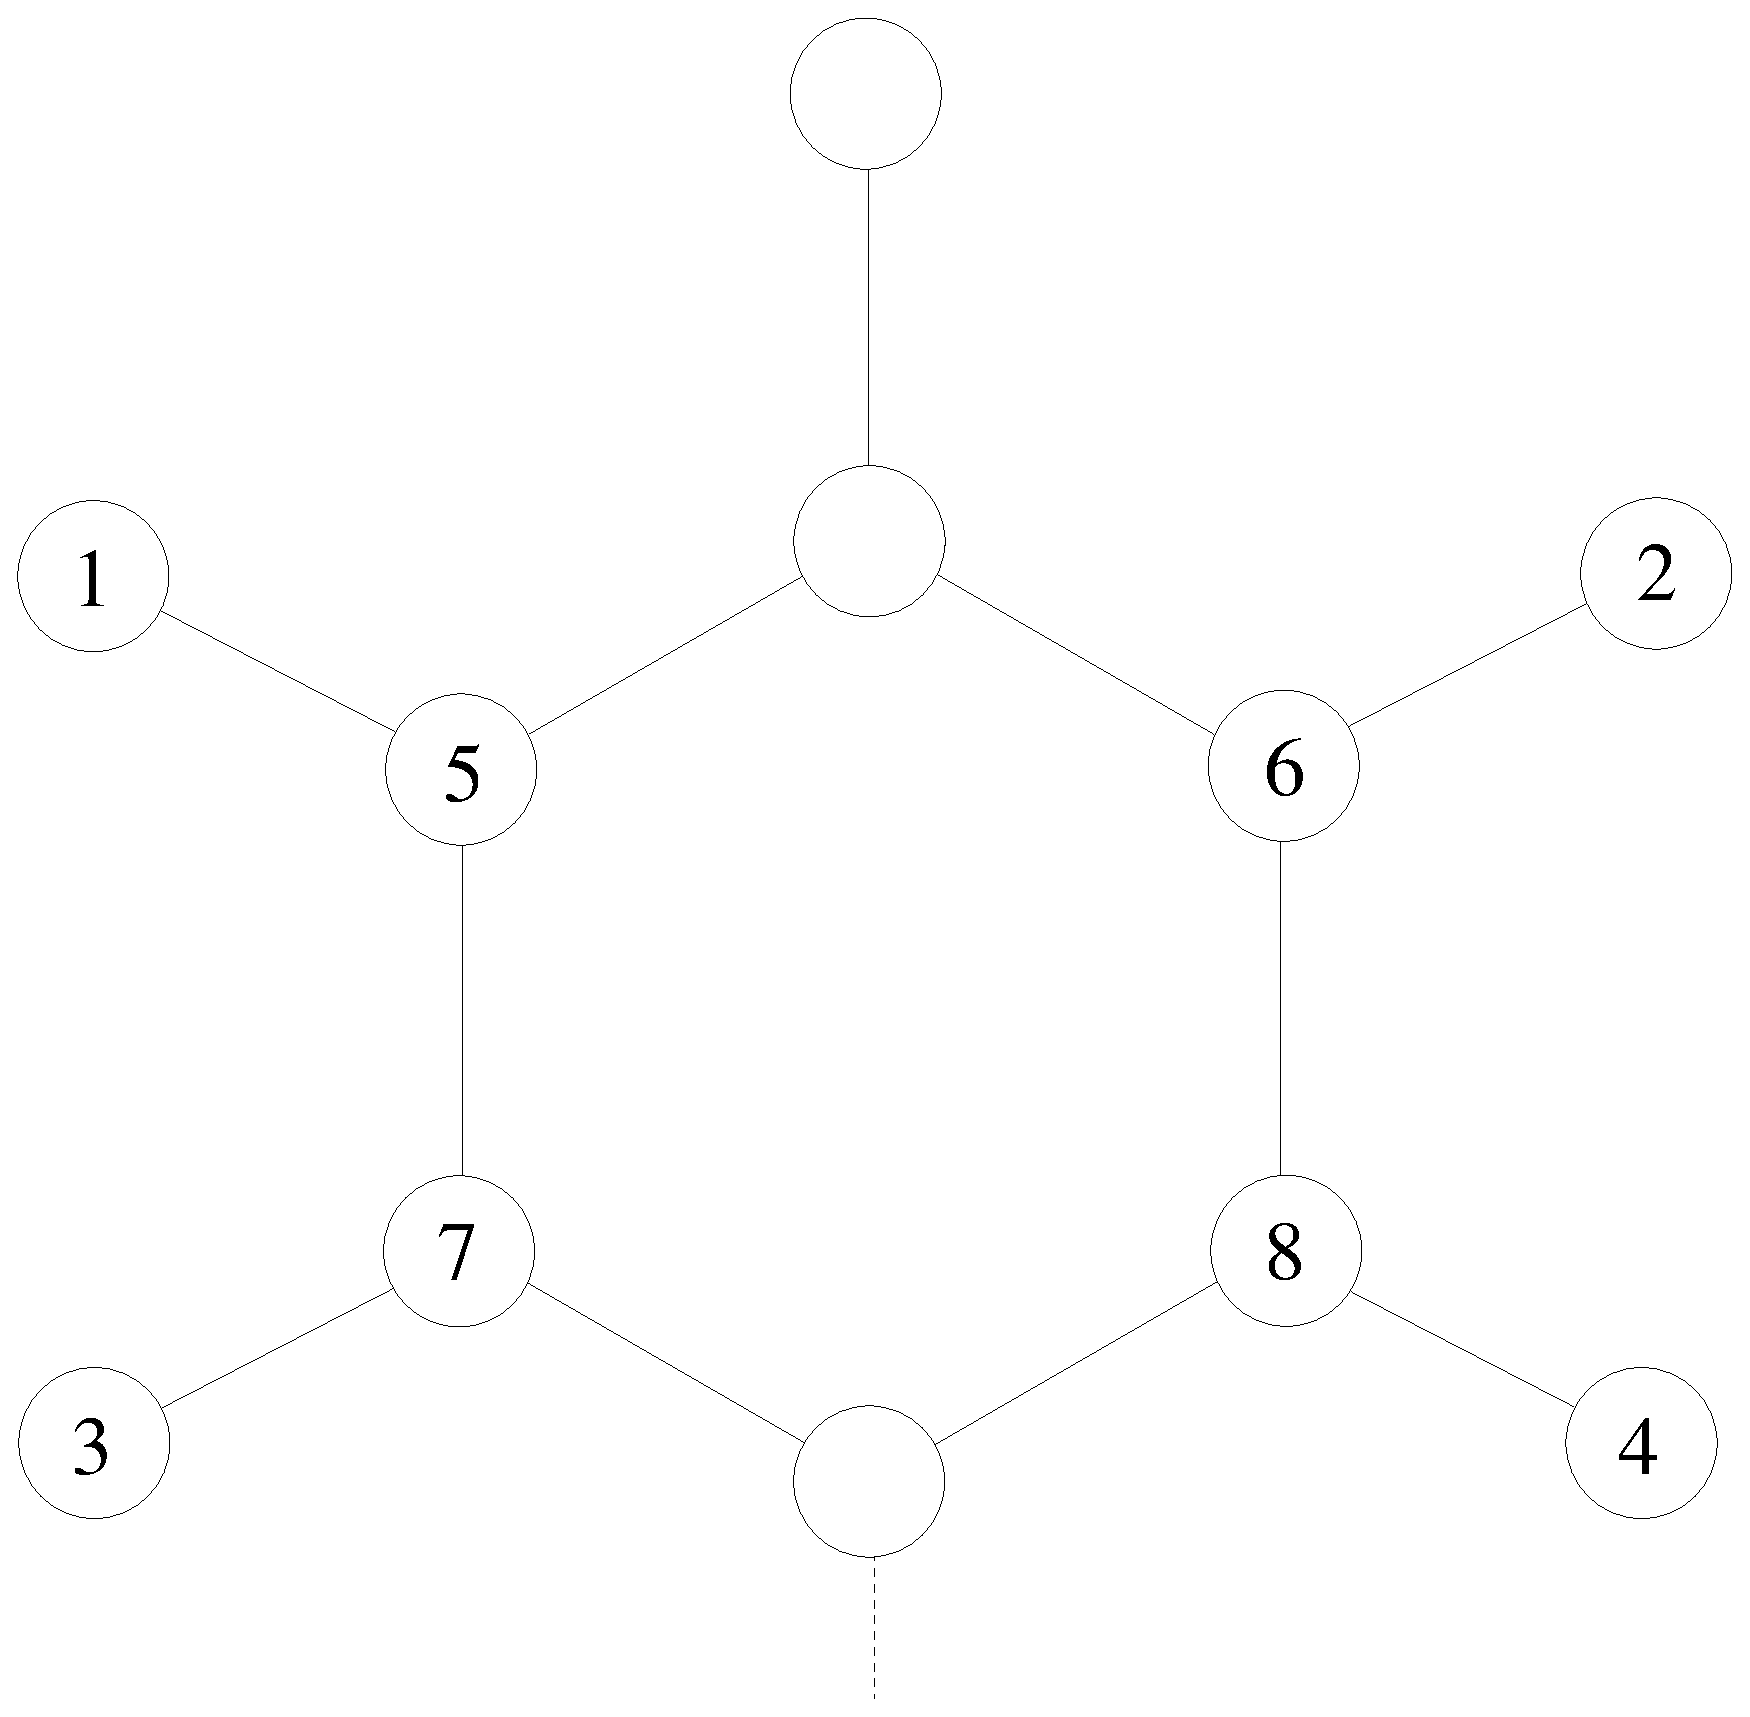
\includegraphics[width=0.5\textwidth]{PHE.eps}}
\end{figure}

For the phenylalanine example illustrated we must allow three other pairs of
atoms to exchange if we swap 7 and 8. Hence a suitable {\tt perm.allow} entry is
{\obeylines
1

2 3

7 8 5 6 1 2 3 4
}
Here $n=2$ and $s=3$: if we exchange 7 and 8 then we must also exchange 5 and 6,
1 and 2, and 3 and 4. There are two atoms in each of the three secondary sets, 
since we have specified 7 and 8 as the two primary atoms.

Here is an example {\tt perm.allow} file for a water trimer using
the flexible {\it QTIP4PF\/} potential, where the energy is invariant to permutations
of water molecules and to exchanges of hydrogens in the same molecule. However,
hydrogens cannot exchange between different oxygens:
{\obeylines
4

3 2

1 4 7 2 3 5 6 8 9

2 0 

2 3

2 0 

5 6

2 0 

8 9
}
The first group of three oxygens has two atoms that must move with each oxygen,
i.e.~atoms 2 and 3 for oxygen 1, etc. Hydrogen permutations for each oxygen are
allowed by the three following groups. This scheme allows atoms to appear in more 
than one group. There must be a group containing each complete set of permutations
in order for permutation-inversion isomers to be recognised. The format
is compatible with an older scheme, where only pair swaps were allowed for
associated atoms, but now allows for more general permutations.

Scripts to generate allowed permutations automatically for CHARMM and AMBER are available from
the group web site. It is essential to use symmetrised versions of the corresponding
force fields! 

\item {\it PERMINVOPT x\/}: minimise the distance between the geometries in
{\tt coords} and {\tt finish} with respect to permutations, as well
as overall translation, rotation, and inversion. See
{\it PERMOPT\/} for distance optimisation without the inversion.
To specify specific groups of
permutable atoms a {\tt perm.allow} file is needed, unless all atoms (or rigid bodies)
are considered permutable.
For rigid bodies the file {\tt rbsymops} can be used to specify symmetry
operations of each molecule, and the distance will then also be
minimised with respect to internal symmetry operations.
To minimise the Euclidean distance between two configurations with no permutations
a {\tt perm.allow} file with the single entry `0' can be used. 
The configurations are then aligned as if they were rigid bodies decorated
with fixed sites.
The parameter {\it x} is the distance tolerance for assigning atoms to orbits
in the {\bf myorient} standard orientation routine, default value 0.001.
If {\it x} is too small it is possible for permutational isomers to be missed,
however, if {\it x\/} is too large then runs with the {\it AVOID\/} keyword can
slow down by an order of magnitude.

\item {\it PERMOPT x\/}: minimise the distance between the geometries in
{\tt coords} and {\tt finish} with respect to permutations, as well
as overall translation and rotation, but not the inversion. To specify specific groups of
permutable atoms a {\tt perm.allow} file is needed, unless all atoms (or rigid bodies)
are considered permutable.
For rigid bodies the file {\tt rbsymops} can be used to specify symmetry
operations of each molecule, and the distance will then also be
minimised with respect to internal symmetry operations.
To minimise the Euclidean distance between two configurations with no permutations
a {\tt perm.allow} file with the single entry `0' can be used. 
The configurations are then aligned as if they were rigid bodies decorated
with fixed sites.
The parameter {\it x} is the distance tolerance for assigning atoms to orbits
in the {\bf myorient} standard orientation routine, default value 0.001.
If {\it x} is too small it is possible for permutational isomers to be missed,
however, if {\it x\/} is too large then runs with the {\it AVOID\/} keyword can
slow down by an order of magnitude.

\item {\it PLUS\/}: when combined with keywords {\it NEON\/} or {\it ARGON\/}
uses a diatomics-in-molecules potential for the singly charged cation.

%\item {\it PMAX max\/}: {\it max\/} is the maximum probability of dihedral angle twisting for {\it AMBER\/}.

%\item {\it PMIN min\/}: {\it min\/} is the minimum probability of dihedral angle twisting for {\it AMBER\/}.

\item {\it POWER ipow\/}: {\it ipow\/} is the initial power for shifts in the old line minimisation routine
for conjugate gradient. LBFGS minimisation should be used instead.

\item {\it PROJI\/}: turns on projection operator to enforce $I$ point group symmetry
in {\bf mylbfgs.f}. The geometry is projected after every proposed step.

\item {\it PROJIH\/}: turns on projection operator to enforce $I_h$ point group symmetry
in {\bf mylbfgs.f}. The geometry is projected after every proposed step.

\item {\it PRTFRQ n\/}: prints the energy every {\it n\/} steps; default is every step.
Should now work for basin-hopping, basin-sampling and parallel tempering runs.

\item {\it PRINT\_PTGRP tol1 tol2 tol3\/}: Print point-group classification and order for each structure saved in the file {\tt lowest\/}. The three tolerances are optional: {\it tol1\/} is a dimensionless tolerance for diagnosing degeneracies in (normalised!) principal moments of inertia, {\it tol2\/} is the distance tolerance used for detecting point-group symmetry operations, and {\it tol3\/} is a dimensionless tolerance used for testing whether a generated rotation matrix (representing a symmetry operation) is new. The default values are $0.001$, $0.2$ and $0.1$, respectively.

\item {\it PRINT\_MINDATA eigen\_tol\/}: Print the energy, log product of (non-zero) Hessian eigenvalues, and the order of point group for each minimum in the file {\tt lowest\/}, instead of the usual comment line. The optional real-valued parameter {\it eigen\_tol\/} sets the tolerance for diagnosing negative (less than {\tt-abs(eigen\_tol)}) or zero Hessian eigenvalues. The default value is {\it eigen\_tol = 0.001\/}. Note that if a negative eigenvalue is diagnosed or if the number of zero eigenvalues is unexpected, then the ``minimum'' will not be written to the file {\tt lowest\/}. 

\item {\it PTMC histmin histmax ptemin ptemax pttmin pttmax exchprob nequil ptsteps nenrper hbins\/}: 
requests a standard parallel tempering MC run.
This keyword also specifies the energy range for the histogram of quench energies,
{\it histmin\/} to {\it histmax\/},
the energy range for the histogram of instantaneous configurations, {\it ptemin} to {\it ptemax}, 
the temperature range ({\it pttmin} and {\it pttmax}), 
the probability of attempting an exchange {\it exchprob}, the 
number of equilibration steps, {\it nequil},
the number of parallel tempering MC steps without quenching,  {\it ptsteps},
the number of bins for the histogram of instantaneous potential energy, {\it nenrper}, and
the number of bins for the histogram of quench energies, {\it hbins}.
Should be used together with the {\it MPI\/} keyword. % and {\it BINSTRUCTURES\/} keywords.
(This option is only available if the source is compiled with an MPI enabled.)  

\item {\it PULL a1 a2 f\/}: apply a static force to the potential, equivalent to adding
the term $V_{\rm pull}=-f(z_{a1}-z_{a2})$. Here $z_{a1}$ and $z_{a2}$ are the $z$
coordinates for atoms $a1$ and $a2$, and $f$ specifies the force.
This potential is designed to simulate a pulling experiment with static force where
a molecule is pulled along the $z$ axis from atoms $a1$ and $a2$.

\item {\it PY sig0 eps0 [cutoff XYZ xbox ybox zbox]\/}: specifies a rigid-body multisite Paramonov-Yaliraki\cite{ParamonovY05} potential with parameters $\sigma_0$ and $\epsilon_0$. Optional arguments are
a cutoff distance in absolute units, a specification of which directions have periodic boundary
conditions, and the size of the periodic box in units of the cutoff. The parameters for and setup
of the rigid body, even if it is just one site, must be specified in a file {\tt pysites.xyz}.

There are two formats for {\tt pysites.xyz}: identical particles and n-ary mixtures. For identical
particles, the format is:
\begin{verbatim}
[number of sites in molecule]
[blank line]
site [x position] [y] [z] shapes [rep coeff] [att coeff] [a11] [a12] [a13] [a21] [a22] a[23] orient [p_x] [p_y] [p_z]
...
site [x position] [y] [z] shapes [rep coeff] [att coeff] [a11] [a12] [a13] [a21] [a22] a[23] orient [p_x] [p_y] [p_z]
\end{verbatim}
For an n-ary mixture,
\begin{verbatim}
0 [the number zero]
[arity]
[blank line]
[number fraction of this type of molecule]
[number of sites in molecule]
[normal site lines]
...
[blank line]
[second number fraction]
[number of sites in second type]
[normal site lines]
...
\end{verbatim}
For example, for a single site molecule,
\begin{verbatim}
1
site 0.0 0.0 0.0 shapes 1.0 1.0 0.5 0.5 0.2 0.5 0.5 0.2 orient 0.0 0.0 0.0
\end{verbatim}

Or, for example, for two-to-one mixture of single sites and pairs,
\begin{verbatim}
0
2

0.66
1
site 0.0 0.0 0.0 shapes 1.0 1.0 0.5 0.5 0.2 0.5 0.5 0.2 orient 0.0 0.0 0.0

0.34
2
site 0.0  0.5 0.0 shapes 1.0 1.0 0.5 0.5 0.2 0.5 0.5 0.2 orient 0.0  0.2 0.0
site 0.0 -0.5 0.0 shapes 1.0 1.0 0.5 0.5 0.2 0.5 0.5 0.2 orient 0.0 -0.2 0.0
\end{verbatim}

%\item {\it QCUTOFF qcut\/}: {\it qcut\/} is a distance cut-off for Coulomb interactions in {\it AMBER\/}.

\item {\it QALCS qalcsmode cutoff\/}: perform Quench-Assisted Local Combinatorial Search to locate a biminimum for a multicomponent system. (More general than {\it HOMOREF\/}, which works only for binary systems.) The search comprises a sequence of quench-assisted atom swaps, where each step involves a sweep through the local neighbourhood structure induced by the ``interchange'' distance metric. There are many ways of doing this: {\it qalcsmode=0\/} specifies a slow steepest-descent-like search in permutation space; whereas modes 1 through 5 specify alternative schemes that are more efficient for larger systems. Modes 4 and 5 admit an additional (optional) integer parameter {\it cutoff}, which specifies that only the first {\it cutoff} entries in the sorted local neighbourhood are to be considered. The sorting is done by approximate swap gain. 

\item {\it QALCS\_SURF\/}: specifies that QALCS should include surface vacancies as a separate species, akin to dynamic-lattice-search-type methods but relies on a different construction of surface vacancies. The scheme constitutes a deterministic way of refining the surface of a cluster within the QALCS framework, and it can be used with or without the
{\it QALCS\/} keyword (for single- or multi-component clusters). Note that during the surface optimisation all particles are treated as being the same.

\item {\it QCIAMBER}: tells QCI to use the topology file information to add constraints 
corresponding to bonded atoms 
(currently only for one chain of AMBER atoms, additional features are work in progress).

\item {\it QCIINT}: if present, check for internal distance minima for atom pairs between
images, and add extra terms to the energy and gradient if detected. This is the quasi-continuous
part of QCI. Default is off.

\item {\it QCIIMAGE imsepmin imsepmax intimage maxintimage intntriesmax intimageincr intimagecheck\/}
specifies the behaviour of interpolation images for the {\it QCI\/}
quasi-continuous interpolation procedure.
{\it intimagecheck\/} (default 25) is the interval for checking the spacing of the interpolation images.
Images separated by less than {\it imsepmin\/} (default 0.2) can be combined, while an
additional image can be added between images further than {\it imsepmax\/} (default 10.0) apart.
{\it intimage\/} is the initial number of images (default 3),
{\it maxintimage\/} is the maximum number of images (default 75),
{\it intntriesmax\/} is the maximum number of quasi-continuous interpolation
attempts for a given pair of minima (default 2), and
{\it intimageincr\/} (default 6) is the increment in the number of initial images for
further connection attempts between minima that have already been tried.
See also
{\it QCIINT\/},
{\it CONCUTABS\/},
{\it CHECKREP\/},
{\it INTFREEZE\/},
{\it QCI\/}, and
{\it MAXCON\/}.

\item{\it QCICONCUT x\/}: specifies the maximum distance between constrained atoms in the
QCI potential.
See also
{\it QCIINT\/},
{\it CHECKREP\/},
{\it INTFREEZE\/},
{\it MAXCON\/},
{\it QCIIMAGE\/}, and
{\it QCI\/}.

\item{\it QCI intconstrainttol intconstraintdel intconstraintrep intconstrainrepcut
intconfrac intconsep intrepsep intsteps1 intconsteps intrelsteps maxcone intrmstol\/}
specifies quasi-continuous interpolation via an auxiliary constraint potential.
{\it intconstrainttol\/} is used to determine constrained distances. The deviation
of the distance between a given pair of atoms
in all reference structures from the average must be less than
{\it intconstrainttol\/}, default 0.1, for this separation to constitute a constraint.
If a percolating network of constraints does not result then {\it intconstrainttol\/}
is increased by 10\% and the analysis repeated.
{\it intconstraintdel\/} multiplies the constraint penalty term in the auxiliary potential,
default 10.0.
{\it intconstraintrep\/} multiplies the repulsive penalty term in the auxiliary potential,
default 100.0.
{\it intconstrainrepcut\/} is the cutoff for the repulsive penalty term in the auxiliary potential,
default 1.7.
{\it intconfrac\/} is the fraction of the true potential used for the second optimisation
phase after the interpolation with the constraint potential has been achieved. The
default value is 0.9.
{\it intconsep\/} is the maximum difference between the order number of atoms for
which constraints are allowed. The default is 15, which seems appropriate for
biomolecules. However, if a {\tt congeom} file of reference minima is specified, or
a corresponding {\tt congeom.dat} file is present, then {\it intconsep\/} can be set
greater than the total number of atoms.
{\it intrepsep} is the minimum difference in order number of atoms for which repulsive
terms are added to the potential. The default is zero; there are no repulsive terms
between constrained atoms.
{\it intsteps1} is the maximum number of minimisation steps allowed for optimisation
of the interpolation potential, default 300000.
{\it intconsteps\/} is the number of additional minimisation steps after interpolation
with the auxiliary potential has been achieved, where the potential is changed to
include a fraction {\it intconfrac\/} of the true potential, default 100.
{\it intrelsteps\/} is the number of minimisation steps allowed after adding an atom
in the interpolation phase before backtracking if the convergence conditions on the
interpolation metric and root mean gradient have not been achieved, default 200.
{\it maxcone\/} is the value of the auxiliary potential below which an interpolation
step is considered converged, default 0.01.
{\it intrmstol\/} is the value of the root mean square gradient for
the auxiliary potential below which an interpolation
step is considered converged, default 0.01.
See also {\it QCIINT\/},
{\it CHECKREP\/},
{\it INTFREEZE\/},
{\it MAXCON\/},
{\it QCIIMAGE\/}, and
{\it KINT\/}.

\item {\it QCIMAXACTIVE n}: sets the maximum number of active atoms allowed in QCI.
Atoms are frozen in order of activation if this threshold is exceeded. 
The default is to allow all atoms to be active.

\item {\it QCIRADSHIFT x}: applies a radial shift around the next added active atom of
magnitude {\it x}. The idea is to help make room for the new atom in the interpolation.
Default is zero.

\item {\it QMAX cgmax\/}: {\it cgmax\/} is the tolerance for the 
RMS force in the final set of quenches that are used to produce
the output for file {\tt lowest}. The default is 
{\it cgmax\/}$=10^{-3}$, but the appropriate value depends upon the system in question.
{\it TIGHTCONV} can be used instead.

\item {\it QUAD\/}: requires documentation.

\item {\it QUCENTRE\/}: sets the centre of coordinates to the origin (0,0,0) before each MC step is taken (so after each quench), but not during the minimisation itself unlike {\it CENTRE}. 

\item {\it RADIUS radius\/}: sets the radius of the container that prevents particles
evaporating during quenches. If unset the program calculates an appropriate value
based upon the volume per particle for close-packed material and the known pair
equilibrium distance for the given potential. The formula employed is
$$  RADIUS=r_e\left[1 + \left(3 n \over 4\pi\sqrt{2}\right)^{1/3}\right], $$
where $n$ is the number of atoms and $r_e$ is the pair equilibrium
separation.\cite{kittel76} The `1' in this formula is to allow some extra space for
more open structures.

\item {\it RANDOMSEED\/}: specifies that the random number generator should be seeded with system time after each quench, allowing simple parallel use. Currently functional only for the CHARMM and AMBER potentials.

\item {\it RANSEED i\/}: integer seed for the random number generator. The number actually used is mod({\it i\/},10000)+1.

\item{\it RANDMULTIPERM n\/}: randomly permute atomic labels every {\it n\/} basin-hopping steps. Intended for use in conjunction with keyword {\it QALCS\/}. 

\item {\it RATIO stepratio tempratio\/}: adjusts stepsize and temperature independently.
{\it stepratio} is the target fraction of steps that move into a different well. Identity of
structures is determined by structural alignment; as such, the {\it PERMDIST} keyword and
appropriate auxiliary files are required. {\it tempratio} is the target acceptance ratio for
those steps that move into new basins. If a negative number is supplied for either, the
ratios is printed, but the corresponding parameter is not adjusted.

\item {\it RBSYM\/}: specifies that internal symmetry operations permuting equivalent sites for
rigid-body building blocks exist. The operations are read in from a file {\tt rbsymops}, which must
exist in the working directory. The first line of the file is an integer that specifies the number
of operations generated by proper axes of rotation including the identity operation; the operations
are then read in one at a time in a representation consisting of a unit vector, defining the
axis in the reference frame, and an angle in degrees, describing the magnitude of rotation about
that axis. The first operation has to correspond to the identity operation.

This keyword has to be combined with {\it PERMDIST\/} so that structures are aligned and
a distance metric considered based on permutations of identical rigid
bodies and any internal symmetry operation of each rigid body that is a symmetry
of the potential energy function.


%\item {\it RCUTOFF rcut\/}: {\it rcut\/} is a distance cut-off in {\it AMBER\/}.

\item {\it RELAXFINALQUENCH\/}: This means final quench is done in atom coordinates. Useful if you want to compare final energies. This is to be used with {\it RIGIDINIT\/} keyword.

\item {\it RESERVOIR n\/}: for use in combination with {\it PTMC}. A reservoir of local minima
is used for the lowest temperature replicas up to cpu number {\it n}. The default is
$n=0$, which means that only the lowest replica used the reservoir. Visit statistics are
dumped for replicas that use the reservoir, but exchanges only occur when the lowest
non-reservoir replica inherits a configuration. This keyword requires files
{\tt min.data} and {\tt points.min} in the current working directory in {\tt PATHSAMPLE}
format. See also {\it EXEQ\/}.

\item {\it RESIZE resize\/}: all the coordinates are multiplied by {\it resize\/} after
they have been read in, before any other operations are performed. This command is useful
for scaling results obtained with one potential for a system with a different pair
equilibrium distance.

\item {\it RESTART\/ nrelax nhs\/}: reseed runs if a step in not accepted
within twice {\it nrelax} steps.
{\it nhs} is the number of hard sphere moves used to produce the new starting configuration.
If {\it nhs=0} (the default) then the geometry is changed by reseeding.

\item {\it RESTORE\/ dumpfile intEdumpfile\/}: restore a previous {\tt GMIN} run from a {\it dumpfile}.
The number of basin-hopping steps performed will be the difference between the number
requested for the run that produced the dumpfile, minus the number that were completed
at the point the dumpfile was created. This option is not available before version 2.3.
If you are using the {\it A9INTE\/} keyword, you can specify the interaction enthalpy
dump file to restore from as a second arguement.

\item {\it RGCL2\/}: specifies a DIM rare gas-Cl$_2$ potential.

\item {\it RIGIDINIT\/}: This will turn on the local rigid body framework. This keyword needs two additional input files: {\it coordsinirigid\/} and {\it rbodyconfig\/}. {\it coordsinirigid\/} should contain the coordinates of all the atoms whether they are part of local rigid bodies or not. During initialization, GMIN will select appropriate coordinates and throw away irrelevant ones. The format is: \\
{\it x1 y1 z1} \\
{\it x2 y2 z2} \\
{\it \ldots} \\
{\it \ldots} \\
{\it xn yn zn} \\

The file {\it rbodyconfig\/} defines the rigid bodies, with the following format: \\
{\it GROUP NoAtomsInGroup} \\
{\it Atom 1} \\
{\it Atom 2} \\
{\it \ldots} \\
{\it \ldots} \\
{\it Atom N} \\
The keywords {\it RELAXFINALQUENCH\/} and {\it NRELAXRIGID\/} can be used in conjuction with {\it RIGIDINIT\/}.

\item {\it RINGROTSCALE factor\/}: when applying cartesian moves with CHARMM, amino acid rings are moved as rigid units. Setting {\it factor} (default 0.0) between 0.0 and 1.0 will apply a random rotation to these rings during step taking. The suggested value is 0.1 to prevent the regular formation of high energy structures. 

\item {\it RKMIN\/}: specifies a Runga-Kutta minimisation scheme. 
Very inefficient.

\item{\it RMS rmslimit rmstol rmssave lca best}: used with {\it CHARMM} keyword to
specify that the RMSD compared to a reference geometry is calculated. The reference geometry must 
be given in xyz-format in an additional file {\tt compare}. {\it rmssave} is an integer 
that specifies the number of lowest energy geometries and RMSD $\le$ {\it rmslimit}
to save. Geometries are only saved if their RMSD's are more than {\it rmstol} 
different. The flag {\it lca} controls whether the all-atom RMSD ({\it lca}=0) or the $C_{\alpha}$-RMSD 
({\it lca}=1) is calculated. The flag {\it best} determines which structure is compared to the reference
after each quench. {\it best}=0 implies the current quench minimum and {\it best}=1 implies the current best (lowest energy) minimum. If {\it TRACKDATA} is also specified, the RMSD calculated after each quench is produced in the file `rmsd' in gnuplot readable format.

\item {\it ROTAMER maxchange pselect occuw (centre cutoff)\/}: Used with AMBER9 only. Specifies that rotamer moves should be taken. Every step, up to {\it maxchange} rotamers may be selected with a probability {\it pselect}. {\it occuw} determines the minimum \% occupation a rotamer must have to be selected from the library\cite{lovelljm00} when making a change. For example, {\it occuw} $= 0.004$ restricts possible rotamer choice to those with a greater than 0.4\% occupation. If you want to focus rotamer changes around a ligand/binding pocket, the optional {\it centre} and {\it cutoff} arguements may be used. {\it centre} specifies the residue of interest (for example a ligand), and {\it cutoff} the limiting distance from this centre that rotamers may be changed. The selection probability decreases linearlly from the {\it centre} residue. To use these moves, you need three files found in the SCRIPTS directory: PdbRotamerSearch, penultimate.lib and rotamermove.csh in your working directory for each run. 

\item {\it ROTATEHINGE freq factor}: For use with the plate-folding potential (but could possibly be used elsewhere as well). An input file {\tt hingeconfig} is used to define hinges between sets of rigid bodies. Every {\it freq} steps, the set of rigid bodies on the ``moving side'' of the hinge are rotated about the hinge axis by a random angle between $-\pi \times factor$  and $\pi \times factor$.

For each hinge, {\tt hingeconfig} contains the following three lines:

\vspace{0.5cm}

{\it nmove}, the number of plates on the ``moving side'' of the hinge

{\it [plate\_indices] }, a list of rigid body indices for the moving plates

{\it atom1 atom2 atom3 atom4}.

\vspace{0.5cm}

The hinge axis connects the midpoints of the lines connecting the two pairs ({\it atom1}, {\it atom2}) and ({\it atom3}, {\it atom4}). For the plate potential, each of these atom pairs should straddle the hinge and be connected by a stiff spring. {\it atom1} lies on the same plate as {\it atom3}. {\it atom2} and {\it atom4} are on the opposite side of the hinge.

\item {\it ROTATERIGID freq factor}: for use with the generalised rigid body framework, 
{\it RIGIDINIT}. Randomly rotates each rigid body in the system by a factor of $2\pi$ multiplied by {\it factor} every {\it freq} steps.

\item {\it SANDBOX\/:} Specifies that the sandbox potential should be used. This keyword requires an auxiliary input file {\tt rbdata} and produces an auxiliary output visualization file {\tt sandout.xyz}. See the Sandbox section of this documentation for information on producing rbdata files and for examples.

\item {\it SAVE nsave\/}: {\it nsave\/} is an integer that specifies the number of lowest
energy geometries to save and summarise in the file {\tt lowest}. 
Arrays are now dynamically allocated, so any positive integer can be specified. Note that if {\it nsave\/} is large, minima that are not in the Markov chain might also be written out which might be high energy non-physical conformations.  

\item {\it SAVEMULTIMINONLY\/}: specifies that only multiminima are to be considered for the final dump to {\tt lowest}.

\item {\it SAVEINTE nsaveinte\/}: {\it nsaveinte\/} is an integer that specifies the number of lowest
interaction enthalpy geometries to save and summarise in the file {\tt intelowest}. See {\it A9INTE\/}. 

\item {\it SEMIGRAND\_MU mu\_1 \dots mu\_M\/}: specifies the semi-grand chemical potentials, relative to the first species, for use in conjunction with the keyword {\it LFLIPS\/}. The number of values ought to match the number of different species minus one (i.e. {\it M=NSPECIES-1}).

\item {\it SETCENTRE x y z\/}: Sets the centre of mass/coordinates (before the initial quench) to ({\it x,y,z\/}). For example, {\it SETCENTRE 0.0 0.0 0.0\/}
would translate the centre of mass to the origin.

\item {\it SETCHIRAL}: For use with {\it AMBER9}, {\it NAB} and {\it AMBER12} keywords. Specifies that the expected chirality of each centre should be
maintained based on that in the initial quenched minimum, rather than the standard chiralities found in most proteins/nucleotides. 
WARNING: Presently for {\it AMBER12}, without this keyword being included, no chirality checking is done at all!

\item {\it SC nn mm sig sceps scc\/}: specifies a Sutton-Chen potential\cite{suttonc90} with
parameters $n=${\it nn\/}, $m=${\it mm\/}, $a$={\it sig\/}, $\epsilon=${\it sceps\/} and 
$c=${\it scc\/}.

\item {\it SEED nsstop\/}: if the {\it SEED\/} keyword appears then the program
looks for a file {\tt seed} containing coordinates, which are used to `seed' the new run.
The number of coordinates given in this file should be no more than one less than the number
given in {\tt coords}. The specified coordinates are frozen from the first step until 
step {\it nsstop\/}.

\item {\it SHIFTCUT\/}: specifies a shifted-truncated potential for bulk binary Lennard-Jones.

%\item {\it SIDESTEP smax\/}: specifies the maximum step in Cartesian coordinates for side-chains
%in {\it AMBER\/}.

\item {\it SLOPPYCONV bgmax\/}: specifies a basin-hopping run (as opposed to standard MC
on the untransformed surface). {\it bgmax\/} is the convergence criterion
for the RMS force in the basin-hopping
quenches. If this criterion is too strict then the run time will be greatly increased.
If it is too sloppy then the performance of the algorithm is impaired. Different values
are needed for different potentials. {\it BASIN} can be used instead.

\item {\it SORT}: for pairwise potentials the atoms can be sorted from most to least
strongly bound. The {\it SORT} keyword enables this sorting for the coordinates printed
in file {\tt lowest}. This can be useful for seeding subsequent runs by removing the
most weakly bound atoms. This sort is not set by default and is meaningless if the
pair energies are not computed.

\item {\it SPECLABELS L1 L2 \dots LM \/}: specifies the labels to be used in file {\tt lowest} for each atomic species. Intended for use with a potential invoked by keywords {\it MLJ\/}, {\it MGUPTA\/} and {\it MSC\/}. Note that each label is interpreted as a string of two characters, and the calculation will stop if the supplied number of labels ({\it M}) does not match the species count.

\item {\it SPECMASS m1 m2 \dots mM\/}: specifies the mass for each atomic species (all masses are 1 by default). Intended for calculation of a mass-weighted Hessian or molecular dynamics simulations. Error will occur if the supplied number ({\it M}) of masses does not match the species count.

\item {\it STAR}: specifies an excited state calculation for Ar$^*_n$ or Ne$^*_n$ for
a diatomics-in-molecules potential when used with {\it NEON\/} or {\it ARGON\/}.

\item {\it STEP step astep ostep block\/}: specifies the maximum step sizes. {\it step\/} is
for the maximum change of any Cartesian coordinate and {\it astep\/} specifies a tolerance
on the binding energy of individual atoms (if available, i.e.~for Morse and LJ) below
which an angular step is taken for that atom. See the following section for more details.
{\it ostep\/} is the maximum displacement of an axis-angle coordinate for a rigid body system
and {\it block\/} (an integer) is the block size for which separate translational and orientational
displacements will be made for rigid bodies. Omitting {\it block\/} or using a value of zero results in
translational and orientational steps being taken simultaneously
for rigid bodies. The default values for {\it step\/},
{\it astep\/} and {\it ostep\/} are all 0.3 and the default value of {\it nblock\/} is zero.

\item {\it STEEREDMIN smink sminkinc smindiststart smindistfinish sminatoma sminatomb\/}: specified steered 
minimisation should be performed (must be used with {\it AMBER9}). For a protein/ligand system, this adds a translation
to the MC move. The vector between the centre of coordinates of groups A and B (as defined in the file movableatoms)
is calculated and set to {\it smindiststart}. During the following minimisation, a restoring force is applied to 
the ligand. The harmonic force constant is initially zero, and rises by {\it sminkinc} every LBFGS step up to a
maximum of {\it smink}. The force is applied until the A-\textgreater B distance is less than {\it smindistfinish}.  

\item {\it STEPS mcsteps tfac\/}: determines the length of the
basin-hopping run through the integer {\it mcsteps\/} and the annealing protocol through
the real variable {\it tfac\/}. The temperature is multiplied by {\it tfac\/}
after every step in each run. 

\item {\it STICKY nrbsites, sigma\/}: specifies a `sticky patch' potential with {\it nrbsites}
sites in the rigid body reference and a value of {\it sigma} for the $\sigma$ parameter.

\item {\it STOCK mu lambda}: specifies a Stockmeyer potential with parameters
$\mu$ and $\lambda$, respectively.

\item {\it STOCKAA muD E\/}: calls a finite system of Stockmayer particles,
where $\mu_{D}$ is the dipole moment strength and the electric field of stength $E$ can be optionally present. The field, if
present, is along the space-fixed z-direction.

\item {\it STRAND}: specifies a system of $\beta$ strands coded using the rigid body formalism.

\item {\it STRESS mode}: calculate and print atomic-level stresses in the file {\tt lowest\/}. The integer parameter {\it mode} is optional, with the default value being 1, when the local pressure and the corresponding anisotropy parameter are printed after each atom's coordinates. Per-atom energy is also printed in the final field. Additional modes can be introduced if other invariants of the local stress tensor are desired.

\item {\it SUPPRESS}: suppresses the majority of the GMIN output.
Think of it as the opposite of {\it DEBUG}.

\item {\it SW\/}: specifies the Stillinger-Weber Si potential.

\item {\it SYMMETRISE int tol1 tol2 tol3 tol4 tol5 qmax mdiff d}: specifies that the symmetrisation
routine should be called every {\it int} steps. The five {\it tol} parameters are tolerances
for various parts of the routine: 
{\it tol1} is used in {\bf ptgrp.f} in defining orbits; 
{\it tol2} is the distance tolerance used in {\bf ptgrp.f} to define point group symmetry operations;
{\it tol3} is the maximum relative difference in principal moments of inertia used to
diagnose point groups with degenerate irreducible representations in {\bf ptgrp.f};
{\it tol4} is the distance cutoff used to determine if a symmetry element has been lost in {\bf symmetry.f}.
Since we are dealing with approximate symmetries, this parameter may be larger than {\it tol2}.
It is compared to the largest atomic displacement divided by the corresponding radius
for the closest permutation.
{\it tol4} is also used to test whether atoms lie on a given symmetry element, and in testing 
whether orbits generated from `floaters' are actually contained in the core.
{\it tol5} is generally to check for atom clashes in {\bf symmetry.f}, including analysis of
missing sites in orbits, as well as overlap between orbits generated from `floaters' and
previous core or new orbit sites.
{\it qmax} is the maximum number of quenches allowed for each call to {\bf symmetry.f}.
{\it mdiff} is used to test whether a generated symmetry operation is new. If any of the nine
components of the corresponding $3\times3$ matrix differs by more than {\it mdiff} from an
existing matrix then the operations are considered to be different.
{\it d} is the exponential factor used in constructing a centre of mass that is biased towards
core atoms. The contribution of each atom is weighted by $\exp(-dx(i))$, where $x$ is the 
centre of mass distance of atom $i$ on the previous cycle.

\item {\it TABOO nlist\/}: specifies a taboo list of the {\it nlist\/} lowest minima should be maintained.

\item {\it TARGET target1 target2 $\cdots$\/}: specifies any number of target energies. 
The current run stops in an orderly
fashion if the current quench energy is within {\it econv\/} of any target (see {\it EDIFF\/}).

\item {\it TEMPERATURE temp\/}: defines the temperature, {\it temp\/}, at which the 
MC runs are conducted. Different values can be specified for serial `parallel' runs if
{\it PARALLEL} is set.
For true parallel basin-hopping use the {\it BHPT\/} keyword and omit {\it TEMPERATURE\/}.

\item {\it TETHER hdistconstraint hwindows ExtrapolationPercent lnHarmFreq}: requests a calculation of the vibrational density of
states for a given minimum. {\it hdistconstraint} is the minimised average radius of the basin of attraction to which the minimum
belongs, {\it hwindows} is the number of potential energy windows into which a WL simulation is split. {\it 
ExtrapolationPercent} is the percentage of the whole potential energy spectrum, for which the density of states is estimated from
the harmonic approximation and not sampled. {\it lnHarmFreq} the log product of positive Hessian
eigenvalues.

\item{\it THOMSON q\/}: specify the Thomson problem for unit charges on a sphere.
If {\it q\/} is present it is taken to be the charge on one particle, which can
therefore be different from all the other unit charges and is read as a real number.

% Doesn't appear to be coded?
% \item {\it THRESHOLD \/}: specifies threshold acceptance of steps. The change in potential energy must be
% less than the value of the {\it TEMPERATURE\/} variable for a step to be accepted.

\item {\it TIGHTCONV cgmax\/}: cgmax is the tolerance for the
RMS force in the final set of quenches that are used to produce
the output for file {\tt lowest}. The default is
{\it cgmax\/}$=10^{-3}$, but the appropriate values depend upon the system in question.
{\it QMAX} can be used instead.

\item {\it TIP n\/}: specifies a TIP{\it n\/}P intermolecular potential for rigid body water molecules.
$\ \le n \le 5$.

\item {\it TOLBRENT tolb\/}: parameter for {\it DBRENT\/} minimisation. 
Inefficient compared to LBFGS.

\item{\it TOMEGA}: used with the {\it CHARMM} keyword to specify that peptide bonds will be twisted along with all other dihedrals.

% \item {\it TN\/}: specifies a truncated Newton minimisation scheme. 
% Inefficient compared to LBFGS.

\item {\it TOSI app amm apm rho\/}: specifies the Tosi-Fumi potential\cite{tosif64}
with parameters $A_{++}$, $A_{--}$, $A_{+-}$ and $\rho$.

\item {\it TRACKDATA}: produces `energy.dat' and `markov.dat' containing the quench number and 
associated energy and markov energy in two columns and `best.dat', containing the current quench number and the current lowest
total energy. If {\it RMS\/} is also specified, a file called `rmsd.dat' is produced containing the RMSD from a reference structure.
See {\it RMS\/} for more information. This allows plotting with gnuplot to monitor convergence of multiple runs.
If {\it A9INTE} is also specified, two additional output files are produced, `intE.dat' containing the quench number and associated interaction
enthalpy, and `bestintE.dat' containing the quench number and current lowest interaction enthalpy. This keyword does not yet function for MPI runs.

\item {\it TRANSLATERIGID freq maxdist}: for use with the generalised rigid
body framework, {\it RIGIDINIT}. Randomly translates each rigid body in the
system by a distance up to {\it maxdist} every {\it freq} steps.

\item {\it TSALLIS q\/}: specifies that steps are accepted/rejected using Tsallis statistics with the
given value of {\it q\/}, rather than the usual Boltzmann condition.

\item {\it TTM3\/}: specifies Xantheas' TTM3-F water potential, coded
by Jeremy Richardson.
The atom order must be O1, O2,\ldots, H1a, H1b, H2a, H2b,\ldots.
The energy is in kcal/mol and the distance unit is \AA.
Hydrogens are NOT permutable between different oxygens.
Note that this potential is prone to cold fusion---setting the {\it COLDFUSION\/}
parameter explicitly may be necessary.

\item {\it TWOPLUS\/}: when combined with keywords {\it NEON\/} or {\it ARGON\/}
uses a diatomics-in-molecules potential for the doubly charged cation.

\item {\it UACHIRAL\/}: MUST be included when using ff03ua, the AMBER united atom forcefield unless you have disabled the checks for inverted chiral carbons
 with {\it NOCHIRALCHECKS\/}. {\it UACHIRAL\/} ensures the correct impropers are used to define sidechain chirality when HB hydrogen is missing. 

\item {\it UNIFORMMOVE\/}: the proposed steps for each atom in {\bf takestep} are uniformly
distributed over a sphere whose radius is adjusted on-the-fly to give the required acceptance
ratio (or fixed if {\it FIXSTEP\/} or {\it FIXBOTH\/} is set).
The default behaviour for backwards compatibility is for the separate $x$, $y$ and $z$ displacements
of each atom to be scaled uniformly within the current step size range.

\item {\it UPDATES nup\/}: {\it UPDATES\/} is the number of previous steps saved in the LBFGS routine,
default 4.

\item {\it UPDATERIGIDREF\/}: Updates the rigid body reference coordinates after a step has been taken when using
{\it RIGIDINIT}. This allows steps to be taken within rigid bodies if required. As unphysical conformations may be introduced
into the rigid bodies this way, {\it HYBRIDMIN} should be allowed these to be relaxed. 

\item {\it USEROT\/}: Include the rigid rotor partition function during a free energy basin-hopping run.

\item {\it VGW ljsigma ljepsilon taumaxsg taumaxfg}: Specifies use of VGW quantum quenching in place of
classical minimization routines such as LBFGS. {\it ljsigma} and {\it ljepsilon} are the corresponding Lennard-Jones
parameters that must be specified, and taumaxsg and taumaxfg are the maximum value of ``imaginary'' time $\tau$ (inverse tempertaure) for the propagation.
The former pertains to the faster ``single-particle'' SP-VGW used for quenching during the MC runs, and the latter for the more accurate
``fully-coupled'' VGW used for the final quenching (analogous to the tight convergence of the LBFGS). A $\tau$ of at least
2.5 is recommended for the SP-VGW and 5.0 for the FC-VGW. A file {\it vgwdata} containing the masses (in a.m.u.) of all particles, in order of the location
of their {\it xyz} coordinates in ``{\it coords}'' must be present (e.g. for a 38 atom Ne cluster, {\it vgwdata} will have 38 lines of ``{\it 20}''). Different
masses are permitted, though the current version allows for only one set of LJ parameters. 

\item{\it VGWCPS on magnitude}: Specifies use of contraining potential for SP-VGW (sloppy convergence), as clusters expand during quantum quenching
with decreasing mass. 1 or 0 for {\it on} corresponds to on/off,
and magnitude should range from 1 to 1000, with 1 having minimal effect, 1000 being highly constrained. Default value is ``on'', with magnitude 1.

\item{\it VGWCPF on magnitude}: Same as VGWCPS but for FC-VGW, used for the final, full quenching (tight convergence).

\item{\it VGWTOL magnitude}: Absolute tolerance parameter for differential equation solver used for VGW quenching. Default value is 0.0001.
For highly quantum or ``stiff'' systems this may need to be increased, while it may be decreased for ``softer'' or less quantum systems to enhance
speed.
 
\item {\it VISITPROP}: if specified the Wang-Landau convergence is governed by proportionality of visits to the current value of
the modification factor, and not the histogram flatness criterion \cite{ZhouB03}.

\item {\it WELCH $A_{++}\ A_{--}\ A_{+-}\ \rho\ Q_+\ Q_-\ \alpha_+\ \alpha_-$\/}: specifies a Welch binary
salt potential with the parameters indicated.

\item {\it ZETT1\/} and {\it ZETT2\/}: specify the Zetterling potentials.
% </kwd>
\end{itemize}

\section{Angular Steps}

For pure pair potentials the total energy can be broken down into a sum of binding
energies for the individual atoms. This is coded for the Morse and LJ potentials.
If the binding energy of any atom is lower than that of the most tightly bound atom
multiplied by the variable {\it astep\/} (see the {\it STEP\/} command above) then
that atom is randomly replaced on the sphere of radius equal to that of the atom furthest
from the centre of mass. Hence if {\it astep\/} is zero angular steps will never be taken,
and the closer this parameter is to one the more atoms will undergo such displacements.
If the step sizes are adjusted to give the required acceptance ratio then both {\it step\/} and
{\it astep\/} are multiplied or divided by $1.05$ every {\it naccept\/} steps depending
upon the current acceptance ratio. If {\it FIXSTEP\/} has been specified then the temperature
is adjusted in the same way and {\it step\/} and {\it astep\/} are unchanged.

% <systems>
\section{Some Recognised Systems}

%\subsection{AMBER}
%
%Specifies the AMBER force field. Coordinates are read from file {\tt coords.amber}.
%See also associated keywords {\it PMAX\/}, {\it PMIN\/}, {\it NMAX\/}, {\it NMIN\/},
%{\it SIDESTEP\/}, {\it RCUTOFF\/}, {\it QCUTOFF\/} and {\it FAKEWATER\/}.

\subsection{Binary Lennard-Jones}

If the {\it BINARY\/} keyword is specified then a binary Lennard-Jones
potential is used\cite{sastryds98}. {\it PERIODIC\/} must also be
specified. Reduced units are used with $\epsilon_{\rm AA}=\sigma_{AA}=1$.
{\it BLJCLUSTER\/} specifies a binary Lennard-Jones cluster.

\subsection{BLN Off-Lattice Protein Model}
\label{sec:BLN}

The general three-colour bead protein model is specified by keyword {\it BLN}.
The potential follows the form described in
{\it Proc.~Natl.~Acad.~Sci.~USA}, {\bf 100}, 10712, 2003, expect that
the coefficients $A_i$, $B_i$, $C_i$ and $D_i$ include a factor of $\epsilon$
explicitly.

{\arraycolsep0pt\begin{eqnarray}
V&\,=\,&\frac{1}{2} K_r\sum_{i=1}^{N-1}(R_{i,i+1}-R_{\rm e})^2
 +\frac{1}{2} K_\theta\sum_i^{N-2}(\theta_i-\theta_{\rm e})^2 \nonumber\\
 &&+\,\epsilon\sum_i^{N-3}\Big[A_i(1+\cos\varphi_i)+B_i(1-\cos\varphi_i) \nonumber\\
  && \qquad +C_i(1+\cos3\varphi_i)+D_i\left(1+\cos\left[\varphi_i+\pi/4\right]\right)\Big] \nonumber\\
 &&+\,4\epsilon\sum_{i=1}^{N-2}\sum_{j=i+2}^N \left[S_{12}\left(\frac{\sigma}{R_{ij}}\right)^{\!12}
    +S_6\!\left(\frac{\sigma}{R_{ij}}\right)^{\!6}\right],
\label{barrelpot}
\end{eqnarray}}
\noindent where $R_{ij}$ is the separation between beads $i$ and $j$ and
the units of distance and energy are $\sigma$ and $\epsilon$, respectively.
The first term represents the bonds linking successive beads in the linear chain, and a 
value of $K_r=231.2\,\epsilon\sigma^{-2}$ was used in most of the work on the 
Honeycutt and Thirumalai frustrated 46-bead model.
The second term is a sum over the bond angles, $\theta_i$, defined by the triplets
of atomic positions ${\bf R}_i$ to ${\bf R}_{i+2}$, and values
$K_\theta=20\,\epsilon\,{\rm rad}^{-2}$ and $\theta_{\rm e}=105^\circ$ were
used for the 46-bead model.
The third term
is a sum over the dihedral angles, $\varphi_i$, defined by the quartets ${\bf R}_i$ to
${\bf R}_{i+3}$. 
In the 46-bead model $A_i=C_i=1.2$ if the quartet involved no more than one N monomer, generating
a preference for the {\it trans\/} conformation ($\varphi_i=180^\circ$), whereas if two or three
N monomers are involved then $A_i=0$ and $C_i=0.2$.
This choice makes the three neutral
segments of the chain flexible and enables them to accommodate turns.
A general specification of these parameters is possible in the new BLN framework
via the auxiliary file {\tt BLNsequence}.
The last term in (\ref{barrelpot}) represents the nonbonded interactions.
In the current BLN implementation $R_{\rm e}$ is set equal to $\sigma$, i.e.~to 
unity in reduced units.

An appropriate {\tt BLNsequence} file for the usual 46-bead model contains the following
lines:

{\obeylines
\noindent comment: $S_{12}>0$ and $S_6<0$ for B-B, L-L and L-B, N-L and N-B and N-N
\noindent 1.0D0 -1.0D0
\noindent 0.33333333333333D0 0.33333333333333D0
\noindent 1.0D0 0.0D0
\noindent comment: coefficients A, B, C, D
\noindent comment: for Helical, Extended and Turn residues in order, four per line
\noindent 0.0D0 1.2D0 1.2D0 1.2D0
\noindent 0.9D0 0.0D0 1.2D0 0.0D0
\noindent 0.0D0 0.0D0 0.2D0 0.0D0
\noindent LBLBLBLBBNNNBBBLBLBBBNNNLLBLLBBLLBNBLBLBLBLNNNLBBLBLBBBL
\noindent EEEEEETEHTHEEEEEEEEHHEHHHHHHHHHHEHTEEEEEEETTTEEEEEEEE
}

\noindent The penultimate line defines the sequence, and the final line
defines which set of $A_i$, $B_i$, $C_i$ and $D_i$ parameters apply to which 
parts of the structure.\cite{BrownFH03}


\subsection{Diatomics-in-Molecules}

At present diatomics-in-molecules (DIM) potentials are available for various
clusters, which are specified by the line {\it ARGON\/}, {\it NEON\/},
{\it ARNO} or {\it RGCL2\/} in {\tt data}.
Further keywords specify the precise nature of the system for argon or
neon clusters: {\it NEUTRAL\/} for ground state neutral
clusters, {\it PLUS\/} for a single positive charge, {\it TWOPLUS\/} for a double positive
charge, {\it STAR\/} for an electronic excited state and {\it DIPOLES\/} for the first order
induction energy in a charged system. Rare gas-Cl$_2$ and Ar$_N$-NO DIM potentials
are specified by the {\it RGCL2\/} keyword.

\subsection{DFT-based tight-binding}

If the {\it DFTB\/} keyword is specified then a DFT-based tight-binding potential
is used. See also the {\it MULTIPLICITY\/} keyword.

\subsection{LB2}

This keyword specifies the potential\cite{LB299a,LB299b,LB204}
\begin{equation}
V = \frac{\epsilon}{2} \sum_{i<j} \left[ \left(\frac{r_{ij}}{\sigma}\right)^2+
\left(\frac{\sigma}{r_{ij}}\right)^2\right],
\end{equation}
where $\epsilon$ and $\sigma$ are set to unity.

\subsection{Farkas}

The Farkas potentials for aluminium and nickel are specified by keywords {\it FAL\/} and
{\it FNI\/}, respectively.

\subsection{Lennard-Jones}

This is the default potential if nothing is specified in {\tt data}. Reduced units are
assumed with $\epsilon=\sigma=1$.

\subsection{Morse}

This potential is specified by the line {\it MORSE rho\/} in {\tt data} and gives a
a Morse potential with $D=r_e=1$. 
The remaining range parameter,\cite{braierbw90,doyewb95,doyew96a} $\rho$, has a default 
value of six.

\subsection{P46}

Keyword {\it P46\/} specifies a 46-bead three-colour model polypeptide. 
See also the more general implementation of the BLN model in \S \ref{sec:BLN}.

\subsection{Stillinger-Weber Si}

Specified by the keyword {\it SW\/}.

\subsection{Sutton-Chen}

These potentials\cite{suttonc90} are specified by the line {\it SC nn mm sig sceps scc\/} in {\tt data},
as described above. 

\subsection{Tight-binding}

Tight-binding potentials for silicon are specified by the keywords {\it MSORIG\/} 
and {\it FRAUSI\/}.
These potentials also understand the 
keywords {\it PERIODIC\/} and {\it CUTOFF\/} which enable calculations on bulk material
to be performed and a cutoff to be imposed on either cluster or bulk calculations.
Keyword {\it ANGSTROM\/} specifies coordinates in \AA ngstrom rather than bohr.

\subsection{TIP{\it n\/}P Water}

The TIP{\it n\/}P intermolecular water potentials are specified by the keyword {\it TIP\/}.
{\it n\/}=1 through 5 are currently coded. For $N$ water molecules the first $N$ lines of
the {\tt coords} file are the coordinates of a reference origin in each of $N$ rigid molecules,
and the next $N$ lines are angle-axis coordinates. The same convention is used in the output
file {\tt lowest}. The lowest minima are also dumped in xyz format in the file {\tt tip.xyz}.

\subsection{Tosi-Fumi}
 
Keyword {\it TOSI\/} specifies a Born-Mayer potential of the form
$$ E = \sum_{i<j}\left[ {q_i q_j\over r_{ij}} + A_{ij}\exp(-r_{ij}/\rho) \right]. $$
The sum runs over all ions. Tosi-Fumi\cite{tosif64} parameters in atomic units should be
entered after the Tosi keyword in the order $A_{++}$, $A_{--}$, $A_{+-}$, $\rho$.
The ions are specified in file {\tt coords} using PL and MI for plus and minus, respectively,
and can be in any order. There need not be equal numbers of positive and negative ions.
Note that the Welch potential has been fitted to include ion polarizabilities and is described below.

\subsection{Welch}This keyword specifies a Welch potential\cite{welchld76,phillipscb91} of the form
\begin{eqnarray*}
% I have tried \bm \boldsymbol etc. but I can't get a bold mu?!
E &= \sum_{i<j}\Bigg[ {\D q_i q_j\over\D  r_{ij}} + A_{ij}\exp(-r_{ij}^{\rm eff}/\rho)
              -{\D q_i({\boldsymbol \mu}_j\cdot{\bf r}_{ij})\over\D  r_{ij}^3}
              -{\D q_j({\boldsymbol \mu}_i\cdot{\bf r}_{ji})\over\D  r_{ij}^3} \\
             &-3{\D   ({\boldsymbol \mu}_i\cdot{\bf r}_{ij})
                   ({\boldsymbol \mu}_j\cdot{\bf r}_{ij})\over\D  r_{ij}^5}
              +{\D  {\boldsymbol \mu}_i\cdot{{\bf{\mu}}}_j\over\D  r_{ij}^3}\Bigg]
              +\sum_i {\D \mu_i^2\over\D 2\alpha_i}, \\
\end{eqnarray*}
where
$$ {\bf r}_{ij}^{\rm eff}={\bf r}_{ij}+{{\boldsymbol \mu}_i\over Q_i}-{{\boldsymbol \mu}_j\over Q_j},
    \qquad r_{ij}^{\rm eff}=\left|{\bf r}_{ij}^{\rm eff}\right|. $$
Welch parameters in atomic units should be
entered after the Welch keyword in the order $A_{++}$, $A_{--}$, $A_{+-}$, $\rho$, $Q_+$,
$Q_-$, $\alpha_+$, $\alpha_-$.
The ions are specified in {\tt coords}  using atom types PL and MI for plus and minus, respectively,
and can be in any order. There need not be equal numbers of positive and negative ions.

% </systems>

\section{{\it SANDBOX} input and output}

The {\it SANDBOX} keyword requires an auxiliary input file {\tt rbdata} and produces an output visualization file {\tt sandout.xyz}. The {\tt coords} file is read in the normal angle-axis fashion: for $N$ rigid bodies, the first $N$ lines are positions and the second $N$ lines are the corresponding angle-axis rotations.

The {\it SANDBOX} potential generates a unary or $n$-ary mixture of rigid bodies (``molecules'') composed of sites. Each site has a molecule-frame position and orientation. The orientation in the molecule frame is specified by an angle-axis rotation. Each site also has an interaction class that specifies how it interacts with sites in other molecules. These interactions are specified in an interaction matrix. A site of interaction class $i$ interacts with a site of interaction class $j$ according to the $(i,j)$-th element of the interaction matrix. This element of the matrix specifies a potential (e.g., LJ, dipole, etc.) and the appropriate parameters (e.g., energy and length scales, dipole strength, etc.).

\subsection{{\tt rbdata}}
All of this information is encoded in the {\tt rbdata}. The file has two parts. The first part specifies the setup of the sites in the molecules, and the second part specifies the interaction matrix. Lines whose first character is \# are comment lines and are ignored.

\subsubsection{Molecule setup}
For unary mixtures, the syntax is
{\tt
\begin{verbatim}
[number of sites in rigid body]

class [interaction class] site [x] [y] [z] orient [px] [py] [pz]
class [interaction class] site [x] [y] [z] orient [px] [py] [pz]
\end{verbatim}
}
where {\tt [x]} is the $x$-coordinates of the site in the molecule frame and {\tt [px]} is the $x$-component of the angle-axis rotation $\vec{p}$ in the molecule frame. For sites with only isotropic interactions, the input for $\vec{p}$ is ignored. For best performance, place the molecule's sites such that the origin corresponds with the molecule's center of mass.

For $n$-ary mixtures, the syntax is
{\tt
\begin{verbatim}
n-ary
[arity]

[number fraction of this species] [optional atom symbol]
[number of sites in this rigid body]
[normal site lines]

[number fraction of this species]
[number of sites in this rigid body]
[normal site lines]

\end{verbatim}
}
The optional atom symbol will cause atoms of different species to have different atom symbols in the output {\tt xyz} file. Default is `O'.

\subsubsection{Interaction matrix}
After skipping a line in {\tt rbdata}, include the interaction matrix using syntax

{\tt
\begin{verbatim}
matrix
[class i] [class j] [potential name] [parameters]
[class i] [class j] [potential name] [parameters]
\end{verbatim}
}
where the potential names and parameters are specified below. The interaction matrix is assumed to be symmetric, so if $(i,j)$ is specified, $(j,i)$ should not be specified.

{\it SANDBOX} will compute certain values that pertain to individual sites only if those sites interact with certain potentials. For example, if a site interacts with some other site according to a dipole interaction, then $\hat{\mu}$ must be computed for both sites. If the row (or column) corresponding to a site's interaction contains only empty or isotropic interactions, however, $\hat{\mu}$ is not computed.

\subsection{Potentials}
\subsubsection{LJ}
{\tt
\begin{verbatim}
[classi] [classj] lj [sigma_0] [epsilon_0] [rep] [att]
\end{verbatim}
}
\begin{equation}
    U_{\mathrm{LJ}} = 4 \epsilon_0 \left[ A \left(\frac{\sigma_0}{r}\right)^{12} - B \left(\frac{\sigma_0}{r}\right)^6\right]
\end{equation}
Here $A$ is the repulsive coefficient and $B$ is the attractive coefficient. For a typical LJ usage, set $A = B = 1$. For a purely repulsive LJ site, set $A = 1$ and $B = 0$. Some potentials (e.g., TIP4P) use values of $A$ and $B$ that are both not equal to $1$.

\subsubsection{Coulomb}
{\tt
\begin{verbatim}
[classi] [classj] coulomb [sigma_0] [k_c] [q_1] [q_2]
\end{verbatim}
}
\begin{equation}
    U_{\mathrm{Coulomb}} = k_C \frac{q_1 q_2}{r}
\end{equation}

\subsubsection{Dipole}
{\tt
\begin{verbatim}
[classi] [classj] dipole [sigma_0] [mu]
\end{verbatim}
}
\begin{equation}
    U_{\mathrm{dipole}} = \frac{\mu^2 \sigma_0^3}{r^3} \left[ \hat{\mu}_i \cdot \hat{\mu}_j - 3\left(\hat{\mu}_i \cdot \hat{r}\right)\left(\hat{\mu}_j \cdot \hat{r}\right)\right]
\end{equation}
where $\mu$ is the dipole strength, $\hat{\mu}_i$ is the dipole orientation of the $i$-th site, $r$ is the distance between sites $i$ and $j$, and $\hat{r}$ is the unit vector pointing between the sites.

\subsubsection{Morse}
\begin{verbatim}
[classi] [classj] morse [eps] [rho] [r_e]
\end{verbatim}
\begin{equation}
    U_{\mathrm{Morse}} = \epsilon \left[1 - \exp\left\{ -\rho \left(r - r_e\right) \right\} \right]^2 - 1
\end{equation}
where $\epsilon$ is the energy scale, $\rho$ is the range parameter, and $r_e$ is the equilibrium bond distance (or length scale).

\subsubsection{Paramonov-Yaliraki}
Pending

\subsection{Example {\tt rbdata} files}
\subsubsection{Normal LJ}
Normal LJ simulations are unary, and the single molecule species has only one site. Although the single site need not be placed at the origin in the molecule frame, putting it anywhere else introduces angular dependencies that will slow down convergence. Because the single site has only isotropic interactions, its orientation is irrelevant, and I leave it as {\tt 0.0 0.0 0.0}.
{\tt
\begin{verbatim}
1

class 1 site 0.0 0.0 0.0 orient 0.0 0.0 0.0

matrix
  # lj sig eps rep att  
1 1 lj 1.0 1.0 1.0 1.0
\end{verbatim}
}
Note that the line beginning with \# is a comment line.

\subsubsection{Binary LJ}
Binary LJ is a 2-ary mixture. The sites in the first species (typically called $A$) are of a different interaction class than the $B$ sites, since the interactions $AA$, $AB$, and $BB$ are all different. This data file can be used to find the global energy minimum for $N=5$.
{\tt
\begin{verbatim}
n-ary
2    # arity 2 -> binary

0.6     # number fraction (5 * 0.6 = 3, which is N_A for global minimum)
1       # number of sites in this type
class 1 site 0.0 0.0 0.0 orient 0.0 0.0 0.0

0.4     # number fraction
1       # number of sites in this type
class 2 site 0.0 0.0 0.0 orient 0.0 0.0 0.0

matrix
  # lj sig eps rep att  
  # AA
1 1 lj 1.0 1.0 1.0 1.0

  # AB
1 2 lj 1.125 1.0 1.0 1.0

  # BB
2 2 lj 1.25 1.0 1.0 1.0
\end{verbatim}
}

\subsubsection{LWOTP}
The LWOTP model consists of three LJ sites arranged in a triangle around the origin. All the sites interact with the same LJ potential, so there is only one interaction class.
{\tt
\begin{verbatim}
3   # three sites

class 1 site  0.0               -0.528902226860823 0.0 orient 0.0 0.0 0.0 #  0.0,        -2/3 sin 7pi/24, 0.0
class 1 site  0.608761429008721  0.264451113430412 0.0 orient 0.0 0.0 0.0 #  cos 7pi/24,  1/3 sin 7pi/24, 0.0
class 1 site -0.608761429008721  0.264451113430412 0.0 orient 0.0 0.0 0.0 # -cos 7pi/24,  1/3 sin 7pi/24, 0.0

matrix
  # lj sig eps rep att
1 1 lj 1.0 1.0 1.0 1.0
\end{verbatim}
}

\subsubsection{TIP4P}
In TIP4P there are three interaction classes: the oxygens interact only with other oxygens, and the two charged sites (hydrogen and lone pairs) interact differently with themselves than with the other.
{\tt
\begin{verbatim}
4   # four sites

class 1  O    0.0         0.0  0.0          orient 0.0 0.0 0.0
class 2  H1   0.756950327 0.0 -0.5858822760 orient 0.0 0.0 0.0
class 2  H2  -0.756950327 0.0 -0.5858822760 orient 0.0 0.0 0.0
class 3  lp   0.0         0.0 -0.15         orient 0.0 0.0 0.0

matrix
  # lj sig eps    rep       att
1 1 lj 1.0 0.25  2510.4d3  2552.24
  # need eps = 1/4 to cancel the 4.0 in the LJ potential
  # rep is kJ angstrom^12 / mol
  # att is kJ angstrom^6 / mol

  # coulomb sig k_c          q_1   q_2
2 2 coulomb 1.0 1389.354848  0.52  0.52
2 3 coulomb 1.0 1389.354848  0.52 -1.04
3 3 coulomb 1.0 1389.354848 -1.04 -1.04
                # k_c is measured in kJ/mol
\end{verbatim}
}

\subsubsection{Stockmayer}
The Stockmayer potential has an anisotropic site. Changing the molecule frame orientation of this site would change the direction of $\hat{mu}$ for the site. In this example, I leave the orientation as {\tt 0.0 0.0 0.0} so that $\hat{\mu}$ is aligned with the molecule frame $\hat{z}$. 
{\tt
\begin{verbatim}
2

class 1 site 0.0 0.0 0.0 orient 0.0 0.0 0.0
class 2 site 0.0 0.0 0.0 orient 0.0 0.0 0.0

matrix
1 1 lj 1.0 1.0 1.0 1.0
2 2 dipole 1.0 1.0
\end{verbatim}
}

\subsection{Output visualization}
{\it SANDBOX} produces a file {\tt sandout.xyz} for visualization. Currently this file places an oxygen (O) molecule at each rigid body's center and supplies an arrow along that rigid body's $\hat{z}$. {\tt sandout.xyz} can be opened with xmakemol.

% <examples>

\section{Example {\tt data} Files}

A basin-hopping run of 10,000 MC steps at reduced temperature $0.8$ for the Lennard-Jones potential
with a constant temperature specified by the `1.0' on the {\it STEPS\/} line.
Seeding occurs for the first 100 steps, so a file {\tt seed} is required in the 
working directory. The final quenches to produce the output in {\tt lowest} are much
tighter than the relatively `sloppy' quenches for the basin-hopping run (compare the
{\it SLOPPYCONV\/} line with the {\it TIGHTCONV\/} line). The maximum number of iterations per
conjugate gradient step is 250 for the sloppy quenches and 500 for the tight quenches.
The initial linear and angular step parameters are 0.36 and 0.4, and these are adjusted
every 50 steps to try and achieve an acceptance ratio of 0.5.

\medskip
\begin{tabular}{ll}
SLOPPYCONV & 0.01 \\
TIGHTCONV & 1.0D-3 \\
SORT \\
MAXIT & 250 500 \\
STEPS & 10000 1.0 \\
STEP & 0.36 0.4 \\
TEMPERATURE & 0.8 \\
\end{tabular}
\medskip

\noindent The next example is similar to the above but employs parameters that seem
to be suitable for a Morse potential with $\rho=6$.

\medskip
\begin{tabular}{ll}
SLOPPYCONV & 0.01 \\
TIGHTCONV & 1.0D-3 \\
SORT \\
EDIFF & 0.01\\
MORSE & 6.0\\
MAXIT & 200 500\\
STEPS & 10000 1.0\\
STEP & 0.35 0.4\\
TEMPERATURE & 0.6\\
\end{tabular}
\medskip

\noindent Global optimisation for a water cluster using the TIP4P potential.
The initial step sizes for translational and orientational rigid-body coordinates are
0.6 and 0.9, respectively, and the block size for separate translational and orientational
steps is 200.

\medskip
\begin{tabular}{ll}
SLOPPYCONV & 0.01 \\
TIGHTCONV & 0.0001 \\
TIP & 4 \\
CENTRE & \\
MAXIT & 1000 1000\\
STEPS & 50000 1.0\\
STEP & 0.6 0.0 0.9 200 \\
TEMPERATURE & 5.0\\
\end{tabular}
\medskip

\noindent The following input file specifies a basin-sampling run to calculate the density of states for 
a LJ$_{13}$ cluster. The system is
confined to a spherical container of radius $1.8\,\sigma$, 
the geometry will be perturbed by $0.2\,\sigma$ at each step with no
angular steps allowed. The run will terminate after $1000000$ 
MC steps or when the WL convergence criterion {\it targetwl}
is satisfied, whichever is the earliest. Setting the temperature to zero indicates that 
a Wang-Landau type MC is used instead of
a conventional temperature-dependent MC run. In keyword {\it HISTOGRAM\/}
the energy of the global minimum of LJ$_{13}$ $-44.3268\,\epsilon$ is chosen
as the energy of the lowest bin {\it histmin}, the energy spectrum above that point is 
separated into $50$ bins of width $0.25$ each. The
starting modification factor and target number of WL iterations are 
{\it histfac} =$ 1.01$ and {\it targetwl} =$ 10$. A square root function
will  be used for decreasing the modification factor upon completion of each WL iteration, 
and the convergence schedule is regulated by {\it VISITPROP}.  


\medskip
\begin{tabular}{ll}
SLOPPYCONV & 0.001 \\
TIGHTCONV & 1.0D-3 \\
MAXBFGS &  0.1 \\
EDIFF & 0.003 \\
RADIUS &  1.8 \\
MAXIT & 1000 500 \\
STEPS & 1000000 1.0 \\
STEP  & 0.2 0.0 \\
TEMPERATURE & 0.0 \\
HISTOGRAM & -44.3268014195 $\:$ 0.2 $\:$ 1.1D0 $\:$ 50 $\:$ 0.5 $\:$ 10 $\:$ 0.2 \\
EQUILIBRATION 1 100 \\
FIXBOTH \\
BINSTRUCTURES 1 \\
VISITPROP \\
\end{tabular}
\medskip

\noindent The following input specifies a local geometry relaxation for a metal (001) surface modelled by the Sutton-Chen potential, smoothly truncated at 2.5\AA. The model parameters are for Ag, and the expected input coordinates are a $[0,5a_{0}] \times [0,5a_{0}] \times [0,X]$ face-centred-cubic slab with the lattice parameter $a_{0} = 1.0$\AA~and $X < 90$\AA. Periodic boundary conditions are imposed in all three dimensions, but the box length in the $z$ direction is made large to create vacuum. The bottom two layers ($z = 0.0$ and $z=0.5$) containing 100 atoms are frozen to mimic an infinite half-space.

\medskip
\begin{tabular}{ll}
TIGHTCONV  & 1.0D-4 \\
SLOPPYCONV & 1.0D-3 \\
MSC & 1 12 6 1.0 1.0 144.41 \\
CUTOFF & 2.5 \\
PERIODIC & 5.0 5.0 100.0 \\
MAXIT & 500 500 \\
STEPS & 0 1.0 \\
STEP & 0.0 0.0 \\
FREEZE & 1 2 3 4 5 6 7 8 9 10 \\
FREEZE & 11 12 13 14 15 16 17 18 19 20 \\
FREEZE & 21 22 23 24 25 26 27 28 29 30 \\
FREEZE & 31 32 33 34 35 36 37 38 39 40 \\
FREEZE & 41 42 43 44 45 46 47 48 49 50 \\
FREEZE & 51 52 53 54 55 56 57 58 59 60 \\
FREEZE & 61 62 63 64 65 66 67 68 69 70 \\
FREEZE & 71 72 73 74 75 76 77 78 79 80 \\
FREEZE & 81 82 83 84 85 86 87 88 89 90 \\
FREEZE & 91 92 93 94 95 96 97 98 99 100 \\
\end{tabular}
\medskip

% </examples>
% <end>
\section{Summary of Major Changes}

\subsection{12/10/10}
Changed to a more flexible scheme for atoms that must move together when
{\it PERMDIST\/} is pecified, in line with OPTIM and PATHSAMPLE.

\subsection{2/11/07}
Implementation of minimum image convention in distance minimisation.
{\it PERMDIST} keyword now made consistent with OPTIM and PATHSAMPLE
using {\tt perm.allow} file.

\subsection{31/12/06}
GMIN.2.3 introduced with MPI support by Tetyana Bogdan and David Wales.
New parallel tempering basin-sampling and
parallel tempering basin-hopping algorithms implemented.

\subsection{18/2/05}
\begin{itemize}
\item GMIN.2.0 recoded in fortran90 by Tetyana Bogdan and DJW. All arrays are now dynamically allocated.
\item Basin-sampling procedure programmed by DJW and developed by Tetyana Bogdan. See the new
{\it HISTOGRAM} keyword.
\item Interface to CHARMM added by David Evans and DJW. See keyword {\it CHARMM} and its associated 
parameters. Internal coordinate minimisation (written by David Evans and developed by Joanne Carr) 
is specified by keyword {\it INTMIN}.
\item Exploitation of approximate symmetry introduced through {\it SYMMETRY} keyword.
\item Bipartite matching implemented for matching closest permutational isomers
(thanks to Tomas Oppelstrup). Now used with 
the {\it PERMDIST} keyword, as well as the new taboo-type procedure introduced through keyword {\it AVOID}.
\item Cooperative moves introduced via keyword {\it COOPMOVE}.
\item Various new potentials have been added: {\it NATB} specifies a tight-binding potential
for sodium (can be guided by {\it GUPTA 21}); various Gupta potentials; Stockmeyer; sticky patches, etc.
\end{itemize}

\subsection{22/6/03}
\begin{itemize}
\item Support for rigid bodies added, e.g.~potentials {\it TIP\/}, {\it CAPSID\/} and {\it OTP\/}.
The centre-of-mass and angle-axis derivatives are calculated in subroutine {\tt rigidfunc.f}, so for pairwise
site-site potentials all that is needed are additional statement functions for these potentials and their
first derivative with respect to the distance.
\item Guiding potentials changed. The new keyword {\it GUIDE\/} allows specification of a parameter,
{\it guidecut\/}, the RMS force below which the real potential is used. 
\item Glue potential for lead added.
\item Keyword {\it TSALLIS\/} introduced for an alternative to the Metropolis
accept/reject step with Boltzmann statistics.
\item Keywords {\it BINARY\/}, {\it BLJCLUSTER\/} and {\it SHIFTCUT\/} introduced for binary LJ systems,
{\it ZETT1\/} and {\it ZETT2\/} for Zetterling potentials, {\it FAL\/} and {\it FNI\/} for Farkas Al and Ni
potentials, {\it ARNO\/}, {\it MULTIPLICITY\/} for {\it DFTB\/} and 
{\it AXTELL\/} for an additive Axilrod-Teller contribution.
Keywords {\it NEWJUMP\/} and {\it PNEWJUMP\/} for parallel runs with parallel tempering-like jumps
and {\it JUMPMOVE\/} for jump-walking parallel runs.
Keyword {\it TABOO\/} for runs with a taboo list.
\item Keyword {\it PERMDIST\/} added for runs that minimise the distance between two structures by permuting
atoms.

\end{itemize}

\subsection{15/10/99}
\begin{itemize}
\item Replaced conjugate gradient minimisation by the limited memory algorithm
      of Jorge Nocedal\cite{lbfgs}.
\item The convergence for {\it SLOPPYCONV\/} and {\it TIGHTCONV\/} is now
      based only on the RMS gradient. The energy change condition has gone.
\item New parameters for the LBFGS routine. {\it PRINTLEVEL\/} sets the 
      print level parameters, {\it UPDATES\/} the number of LBFGS updates
      before resetting and {\it GTOL\/} the tolerance for line minimisation.
\end{itemize}

\def\aciee{Angew.~Chem.~Int.~Ed.~Engl.}
\def\acp{Adv.~Chem.~Phys.}
\def\acr{Acc.~Chem.~Res.}
\def\ac{Acta.~Crystallogr.}
\def\ajp{Am.~J.~Phys.}
\def\am{Adv.~Mater.}
\def\apl{Appl.~Phys.~Lett.}
\def\ap{Ann.~Physik}
\def\Pa{Physica A}
\def\arpc{Ann.~Rev.~Phys.~Chem.}
\def\bbpc{Ber. Bunsenges. Phys. Chem.}
\def\bc{Biochemistry}
\def\cccc{Coll.~Czech.~Chem.~Comm.}
\def\cj{Comput.~J.}
\def\cpc{Comp.~Phys.~Comm.}
\def\cpl{Chem.~Phys.~Lett.}
\def\cp{Chem.~Phys.}
\def\crev{Chem.~Rev.}
\def\dalton{J.~Chem.~Soc., Dalton Trans.}
\def\el{Europhys.~Lett.}
\def\faraday{J.~Chem.~Soc., Faraday Trans.}
\def\fartrans{J.~Chem.~Soc., Faraday Trans.}
\def\fdisc{J.~Chem.~Soc., Faraday Discuss.}
\def\ic{Inorg.~Chem.}
\def\ijmpc{Int.~J.~Mod.~Phys.~C}
\def\ijqc{Int.~J.~Quant.~Chem.}
\def\jacers{J. Am. Ceram. Soc.}
\def\jacs{J.~Am.~Chem.~Soc.}
\def\jap{J.~Appl.~Phys.}
\def\jas{J.~Atmos.~Sci.}
\def\jcc{J.~Comp.~Chem.}
\def\jce{J.~Chem.~Ed.}
\def\jcis{J.~Colloid Interface Sci.}
\def\jcp{J.~Chem.~Phys.}
\def\jcscc{J.~Chem.~Soc., Chem.~Commun.}
\def\jcsft{J.~Chem.~Soc., Faraday Trans.}
\def\jetp{J.~Exp.~Theor.~Phys.~(Russia)}
\def\jmc{J.~Math.~Chem.}
\def\jmsp{J.~Mol.~Spec.}
\def\jmst{J.~Mol.~Structure}
\def\jncs{J.~Non-Cryst.~Solids}
\def\jpa{J.~Phys.~A}
\def\jphysc{J.~Phys.~C}
\def\jpca{J.~Phys.~Chem.~A}
\def\jpcb{J.~Phys.~Chem.~B}
\def\jpcm{J.~Phys.~Condensed Matter.}
\def\jpcssp{J.~Phys.~C: Solid State Phys.}
\def\jpcs{J.~Phys.~Chem.~Solids.}
\def\jpc{J.~Phys.~Chem.}
\def\jpfmp{J.~Phys.~F, Metal Phys.}
\def\jpsj{J.~Phys.~Soc.~Jpn.}
\def\jsp{J.~Stat.~Phys.}
\def\mg{Math.~Gazette}
\def\molphys{Mol.~Phys.}
\def\molp{Mol. Phys.}
\def\mrsb{Mater.~Res.~Soc.~Bull.}
\def\msr{Mater.~Sci.~Rep.}
\def\nat{Nature}
\def\njc{New J.~Chem.}
\def\pac{Pure.~Appl.~Chem.}
\def\phys{Physics}
\def\pla{Phys.~Lett.~A}
\def\phm{Philos. Mag.}
\def\pma{Philos.~Mag.~A}
\def\pmb{Philos.~Mag.~B}
\def\pml{Philos.~Mag.~Lett.}
\def\pnasu{Proc.~Natl.~Acad.~Sci.~USA}
\def\pnas{Proc.\ Natl.\ Acad.\ Sci.\  USA}
\def\pra{Phys.~Rev.~A}
\def\prbcm{Phys.~Rev.~B}
\def\prb{Phys.~Rev.~B}
\def\prc{Phys.~Rev.~C}
\def\prd{Phys.~Rev.~D}
\def\prep{Phys.~Reports}
\def\pre{Phys.~Rev.~E}
\def\prl{Phys.~Rev.~Lett.}
\def\prsa{Proc.~R.~Soc.~A}
\def\pr{Phys.~Rev.}
\def\psfg{Proteins: Struct., Func.~and Gen.}
\def\pssb{Phys.~State Solidi B}
\def\pss{Phys.~State Solidi}
\def\rmp{Rev.~Mod.~Phys.}
\def\rpp{Rep.~Prog.~Phys.}
\def\sci{Science}
\def\ss{Surf.~Sci.}
\def\tca{Theor.~Chim.~Acta}
\def\tetra{Tetrahedron}
\def\zfpd{Z.~Phys.~D}
\def\zpb{Z.~Phys.~B.}
\def\zpc{Z.~Phys.~Chem.}
\def\zpdamc{Z.~Phys.~D}
\def\zpd{Z.~Phys.~D}


\cleardoublepage
\phantomsection
\addcontentsline{toc}{chapter}{Bibliography}

\bibliographystyle{thesis}
\bibliography{GMINdoc}

\end{document}
% </end>
% </document>
